\documentclass[11pt,a4paper]{article}
\usepackage[utf8]{inputenc}
\usepackage[T1]{fontenc}
\usepackage[french]{babel}
\usepackage{lmodern}
\usepackage{amsmath,amssymb}
\usepackage{graphicx,booktabs,array}
\usepackage{xurl}
\usepackage[margin=2.2cm]{geometry}
\usepackage{float,microtype,needspace}
\usepackage[section]{placeins}
\usepackage[colorlinks=true,linkcolor=blue,urlcolor=blue,citecolor=blue]{hyperref}
\graphicspath{{../support/}{figures/}}
% Valeurs issues des calculs complets en différences finies.
\newcommand{\BoundaryReflectingCost}{3,480820}
\newcommand{\BoundaryOpenCost}{0,208522}
\newcommand{\BoundaryMaterialCost}{0,416078}
\newcommand{\BoundaryOpenError}{3,916}
\newcommand{\GradientRelativeError}{\ensuremath{8{,}01\times10^{-8}}}
\newcommand{\RecommendedLevel}{0}
\newcommand{\RecommendedMaterial}{laine de verre}
\newcommand{\RecommendedBandCost}{0,627376}
\newcommand{\RecommendedCoveredNodes}{38}
\newcommand{\RecommendedRobinNodes}{128}
\newcommand{\PlanPeakFrequency}{150}
\newcommand{\PlanPeakCost}{7,141585}
\newcommand{\MonoExampleFrequency}{250}
\newcommand{\MultiBandLevelTwo}{0,942893}
\newcommand{\InitialBandLevelTwo}{1,290230}
\newcommand{\ProfileFrequency}{400}
\newcommand{\FullCostLevelZero}{0,416078}
\newcommand{\FullCostLevelOne}{0,515656}
\newcommand{\FullCostLevelTwo}{0,822255}
\newcommand{\FullCostLevelThree}{1,352007}
\newcommand{\ConfigInitialBand}{1,290230}
\newcommand{\ConfigContinuousBand}{0,476070}
\newcommand{\ConfigBinaryBand}{0,942893}
\newcommand{\ConfigMixedBand}{0,891418}
\newcommand{\ConfigFullBand}{0,822255}
\newcommand{\SelectedBandReduction}{50,95}
\newcommand{\SelectedMaximumReduction}{75,56}
\newcommand{\BestMaximumValue}{7,270847}

\setcounter{tocdepth}{2}
\setlength{\parindent}{0pt}
\setlength{\parskip}{5pt plus 1pt minus 1pt}
\setlength{\intextsep}{10pt plus 2pt minus 2pt}
\setlength{\textfloatsep}{12pt plus 2pt minus 2pt}
\setlength{\abovecaptionskip}{5pt}
\setlength{\belowcaptionskip}{0pt}
\setlength{\emergencystretch}{2em}
\AddToHook{cmd/section/before}{\Needspace{6\baselineskip}}
\AddToHook{cmd/subsection/before}{\Needspace{5\baselineskip}}
\newcommand{\dd}{\,\mathrm{d}}
\newcommand{\ii}{\mathrm{i}}
\newcommand{\code}[1]{\begingroup\def\UrlBreaks{\do\_\do\/\do\.}\nolinkurl{#1}\endgroup}
% Valeurs du calcul fréquentiel effectivement exécuté.
\newcommand{\frequencePic}{400}
\newcommand{\energiePic}{10,8487}
\newcommand{\energieBande}{4416,120}
\hypersetup{pdftitle={ResoniCS -- Optimisation acoustique d'un mur antibruit pour le RER B},pdfauthor={Antoine MARCHE (VT), Joachim BRET   (VT), Olympia MIQUEL, Mathis MORET-BAILLY, Yann MOUSSU}}

\begin{document}
\hypersetup{pageanchor=false}
\begin{titlepage}
\centering
{\Large CentraleSupélec\par}
\vspace{2cm}
{\Huge\bfseries ResoniCS\par}
\vspace{1cm}
{\LARGE\bfseries Optimisation acoustique\\[0.2cm]d'un mur antibruit pour le RER B\par}
\vspace{1.2cm}
{\large Projet d'enseignement d'intégration --- Contrôle des ondes\par}
\vspace{0.6cm}
{\large Année universitaire 2026--2027\par}
\vfill
{\large Auteurs : Antoine MARCHE (VT), Joachim BRET (VT), Olympia MIQUEL, Mathis MORET-BAILLY, Yann MOUSSU\par}
\vspace{1cm}
\end{titlepage}
\hypersetup{pageanchor=true}

\begingroup
\small
\setlength{\parskip}{0pt}
\tableofcontents
\endgroup
\newpage

\section{Introduction}
Le trafic ferroviaire produit des nuisances sonores dont les mécanismes varient avec le fonctionnement du train et son interaction avec la voie. Dans un tunnel ou une tranchée couverte, les réflexions sur les parois peuvent renforcer certaines oscillations. Le projet ResoniCS étudie un panneau destiné à agir sur ce champ acoustique, en prenant le RER B comme cas d'usage.

On cherche à associer une géométrie de paroi et une répartition de matériau poreux pour diminuer un indicateur d'énergie du champ sonore. La comparaison tient compte de la quantité de matériau utilisée. L'objectif est de comprendre où le matériau est utile, puis de rechercher une répartition adaptée à plusieurs fréquences.

Le travail rassemble la formulation du problème, l'identification de coefficients de matériaux, la résolution de Helmholtz par différences finies et l'analyse des placements obtenus par descente de gradient. Les membres de voie théorique ont travaillé sur les propriétés du modèle et la dérivée du critère, en lien avec les membres de voie numérique pour leur mise en œuvre et les tracés. Le programme de référence est organisé en préparation des données, calculs et présentation des résultats.

On commence par un essai à une fréquence, puis on compare les spectres de plusieurs formes, des placements monofréquences et multifréquences, et plusieurs quantités d'absorbant. Les mélanges de matériaux et les profils d'entrée sont ensuite examinés. Le choix final repose sur une comparaison complémentaire avec un même budget de points garnis pour les différentes formes. Tous les résultats annoncés ci-dessous correspondent aux calculs exécutés avec les paramètres indiqués.
\section{État de l'art et cas d'usage}
\subsection{Origines du bruit ferroviaire}
La synthèse initiale de l'équipe distingue trois contributions utiles pour organiser l'étude \cite{sota}. Le \textbf{bruit de traction et des équipements} rassemble notamment les moteurs, la ventilation et les auxiliaires. Le \textbf{bruit de roulement} provient de l'interaction roue--rail. Le \textbf{crissement en courbe} correspond à des oscillations souvent tonales, c'est-à-dire concentrées autour de certaines fréquences, dont l'apparition dépend du contact roue--rail.

Lee et ses coauteurs ont étudié plusieurs liaisons ferroviaires aéroportuaires, dont le RER B \cite{lee2022}. Leurs spectres montrent des contributions aux basses fréquences, notamment autour de 100, 200 et 300 Hz selon la pondération considérée. Ces mesures ont été réalisées \emph{dans les rames}. Elles renseignent le bruit intérieur et ne constituent pas un spectre mesuré au niveau d'un panneau extérieur.

Sur d'autres réseaux de métro, Song et ses coauteurs observent des contributions roue--rail autour de 630 et 2\,500 Hz pour un type de matériel et autour de 800 Hz pour un autre \cite{metro2026}. Les désignations de ces matériels ne renvoient pas aux lignes du RER. L'étude de Kim et ses coauteurs décrit également plusieurs composantes de crissement et de contact en courbe \cite{kim2019}. Leur fréquence dépend du cas étudié. Ces publications motivent des ordres de grandeur pour notre modèle, sans déterminer à elles seules les paramètres d'une source extérieure du RER B.

\subsection{Panneaux réfléchissants, absorption et géométrie}
Un écran acoustique traditionnel modifie la propagation en faisant obstacle à l'onde. Une partie du son est réfléchie et une autre peut contourner l'écran par diffraction. Dans un milieu confiné, les réflexions sur les différentes parois jouent donc un rôle important. La condition de paroi parfaitement réfléchissante utilisée ici représente une idéalisation de ce comportement.

Un matériau poreux comporte des pores dans lesquels le mouvement de l'air s'accompagne de pertes. Son effet peut être représenté par une condition aux limites complexe, dont les paramètres dépendent du matériau et de la fréquence \cite{cours}. On peut ainsi comparer une paroi entièrement recouverte et une paroi partiellement garnie, puis rechercher les zones où une quantité fixée de matériau est la plus utile.

Le cours et la présentation de Filoche décrivent l'intérêt de frontières irrégulières pour la localisation des ondes \cite{cours,filoche}. La \textbf{localisation} désigne une concentration spatiale du champ dans certaines régions. Une géométrie préfractale, obtenue après un nombre fini de répétitions d'un motif, peut modifier les zones de forte oscillation et leur interaction avec le matériau. L'augmentation du contour constitue une motivation pour tester ces formes ; leur efficacité pour notre cas est évaluée par les comparaisons numériques.

\subsection{Solutions développées par les acteurs ferroviaires}
Les écrans installés le long des voies associent plusieurs fonctions. Ils font obstacle à la propagation directe et leur parement peut absorber une partie du son. SNCF Réseau décrit notamment l'emploi de béton-bois, de béton bas carbone et de panneaux métalliques intégrant de la laine minérale \cite{sncfbruit}. Le choix tient aussi compte de la durabilité et de l'intégration dans le site. L'isolation des façades et les interventions sur la voie constituent des actions complémentaires, ce qui montre qu'un panneau répond à une partie du problème ferroviaire.

DELTABLOC propose l'écran bas \emph{Quie@Rail}, dans sa gamme PHONOBLOC \cite{quierail}. Le fabricant décrit des éléments préfabriqués en béton de granulats légers à structure ouverte, placés près de la voie. La configuration annoncée atteint 50 cm au-dessus du plan de roulement et se situe à 2,10 m de l'axe de la voie. Cet exemple montre l'intérêt d'intercepter le bruit près de la zone roue--rail tout en associant la forme de l'écran à un matériau absorbant. Ces dimensions caractérisent ce produit et ne fixent pas celles de notre domaine numérique.

Phononic Vibes développe de son côté \emph{MetaWindow}, un panneau transparent présenté comme absorbant et certifié pour le réseau allemand, en collaboration avec Deutsche Bahn \cite{metawindow}. L'entreprise indique une première installation sur le S-Bahn de Hambourg. La transparence permet de prendre en compte une contrainte d'intégration visuelle en plus de la réponse acoustique. Ces informations proviennent de la présentation du fabricant. Elles illustrent l'existence de solutions industrielles innovantes, sans fournir un gain directement comparable à notre indicateur d'énergie dans un tunnel bidimensionnel.

\subsection{Travaux de recherche sur la forme et le placement de l'absorbant}
Félix, Sapoval, Filoche et Asch ont étudié numériquement des cavités contenant un milieu dissipatif séparé de l'air par une interface irrégulière \cite{felix2009}. Certains modes présentent un champ significatif à la fois dans l'air, où l'onde est excitée, et dans la région absorbante, où l'énergie est dissipée. Leur couplage à ces deux régions peut ainsi favoriser l'absorption. Ce mécanisme explique pourquoi la forme de l'interface joue un rôle, en plus de la quantité de matériau. Il motive l'étude de contours préfractals sans imposer qu'un contour plus irrégulier soit toujours meilleur pour toute excitation.

Magoulès, Nguyen, Omnes et Rozanova-Pierrat proposent un modèle de Helmholtz avec dissipation sur la frontière pour rechercher une forme absorbante \cite{magoules2021}. Ils relient aussi le coefficient complexe de Robin à un modèle où les pertes se produisent dans le volume du matériau poreux. Cette étape est utile à notre projet car le coefficient de paroi doit représenter un matériau documenté avant de permettre une comparaison physique des panneaux.

Magoulès, Menoux et Rozanova-Pierrat étudient ensuite le placement d'une quantité fixée d'absorbant sur une frontière donnée \cite{magoules2025}. Ils établissent un cadre d'optimisation et emploient une descente de gradient pour diminuer l'énergie sur plusieurs fréquences. Dans leurs exemples numériques, une répartition optimisée utilisant 50\,\% d'absorbant peut donner un indicateur d'énergie plus faible qu'une frontière entièrement absorbante. Ce résultat concerne les géométries, les coefficients et la bande de leur étude. Il fournit une hypothèse à tester pour notre cas d'usage, plutôt qu'une performance déjà obtenue pour le RER B.

\subsection{Positionnement de l'étude ResoniCS}
Ces réalisations distinguent trois choix complémentaires : le matériau, la forme du mur et la position des portions absorbantes. ResoniCS reprend cette démarche à l'échelle d'un modèle étudiant. On utilise d'abord les caractéristiques de la laine de roche pour calculer un coefficient de paroi, puis on recherche une répartition à quantité imposée. Les formes planes et préfractales sont comparées avec une même source et une même bande. Les références entièrement recouvertes servent de points de comparaison, avec leur quantité propre annoncée. L'objectif est d'identifier les choix utiles au modèle et de justifier leur effet par les courbes.

\section{Modèle acoustique et géométries}
\subsection{Domaine, pression et conditions aux limites}
On note $\Omega\subset\mathbb R^2$ le domaine occupé par l'air. Sa frontière est décomposée en un bord supérieur $\Gamma_D$, deux côtés réfléchissants $\Gamma_N$ et une paroi inférieure $\Gamma_R$. Le vecteur $n$ est la normale extérieure au domaine et $\partial_nu=\nabla u\cdot n$ désigne la dérivée dans cette direction.

À la fréquence $f$, en hertz, $u_f$ représente l'amplitude complexe de pression. Avec $t$ en secondes et $x$ la position dans le domaine, on écrit
\begin{equation*}
p(x,t)=\operatorname{Re}\!\left(u_f(x)e^{-\ii\omega t}\right)
\qquad \omega=2\pi f
\qquad k_f=\frac{\omega}{c}
\end{equation*}
La pulsation $\omega$ est en radians par seconde et le nombre d'onde $k_f$ en $\mathrm{m^{-1}}$. La célérité vaut $c=343\,\mathrm{m\,s^{-1}}$. La densité $\chi$ décrit la présence d'absorbant sur le mur, avec zéro pour une portion réfléchissante et un pour une portion garnie. Des valeurs intermédiaires sont admises pendant la recherche numérique. La fonction $g$ impose l'excitation à l'entrée et le coefficient complexe $\alpha$ représente le matériau. Le modèle utilise la convention du polycopié \cite{cours}
\begin{equation*}
\begin{cases}
\Delta u_f+k_f^2u_f=0 & \text{dans }\Omega\\
u_f=g(y,\omega) & \text{sur }\Gamma_D\\
\partial_nu_f=0 & \text{sur }\Gamma_N\\
\partial_nu_f+\alpha(\omega)\chi u_f=0 & \text{sur }\Gamma_R
\end{cases}
\end{equation*}
Les tableaux Python \code{f}, \code{f_neu} et \code{f_rob} sont nuls dans ces études. Le tableau \code{f_dir} impose la source $g$. Le symbole $f$ du rapport désigne la fréquence en hertz, que les fonctions de calcul notent \code{frequency_hz}.

Les conditions de Dirichlet, Neumann et Robin désignent respectivement une valeur imposée du champ, de sa dérivée normale, et une relation entre ces deux grandeurs. Ici les parois de Neumann sont rigides et réfléchissantes. Dans le code, \code{Alpha} est le coefficient complexe et \code{alpha_rob} le tableau \code{Alpha*chi}. Le coefficient est exprimé en $\mathrm{m^{-1}}$ pour les coefficients unitaires et les longueurs en mètres.

\subsection{Propriétés de la solution}
Un problème est bien posé lorsque sa solution existe, est unique et dépend continûment des données. Cette dernière propriété signifie qu'une petite modification de l'excitation produit une petite modification du champ, avec une constante qui dépend du domaine et de la fréquence. Les contours préfractals de niveau fini sont polygonaux. Ils relèvent des domaines à frontière Lipschitz du théorème 7.4.3 du polycopié, c'est-à-dire de frontières décrites localement par une fonction à pente bornée \cite{cours}.

Le théorème suppose des données suffisamment régulières, une portion de Dirichlet de longueur positive et les signes
\begin{equation*}
\operatorname{Re}\alpha>0
\qquad \operatorname{Im}\alpha<0
\qquad 0\leq\chi\leq1
\end{equation*}
On suppose aussi que $\chi$ reste supérieure à un nombre strictement positif sur une portion de mur de longueur positive. Une répartition binaire avec une portion garnie satisfait cette condition. La remarque du même paragraphe traite une pression imposée non nulle en écrivant $u_f=\widehat u_f+\widehat g$, où $\widehat g$ prolonge $g$ dans le domaine et $\widehat u_f$ est nul sur $\Gamma_D$. Les seconds membres sont alors modifiés. Le programme impose directement $g$ sur le bord.

Le bilan temporel du §3.2.3 explique le signe dissipatif du coefficient. La variation de l'énergie du problème homogène associé contient un terme proportionnel à $\int_{\Gamma_R}\operatorname{Im}\alpha\,\chi\,|\partial_tp|^2\dd s$, qui est négatif ou nul. Dans nos calculs fréquentiels, on mesure plutôt l'intégrale du module de pression au carré, définie plus loin comme critère de comparaison. L'existence de la solution continue et la précision du calcul sur une grille constituent deux questions distinctes.

\subsection{Mur plan et contours préfractals}
Le générateur \code{create_motif_koch} remplace un segment par huit segments orthogonaux quatre fois plus courts. \code{create_fractal_nodes} répète ce motif, puis \code{_set_geometry_of_domain} marque l'air, les bords et les points extérieurs. On compare le mur plan de niveau zéro et les contours de niveaux un, deux et trois. La figure~\ref{fig:geometries} montre les domaines réellement utilisés.

\begin{figure}[!htbp]
\centering
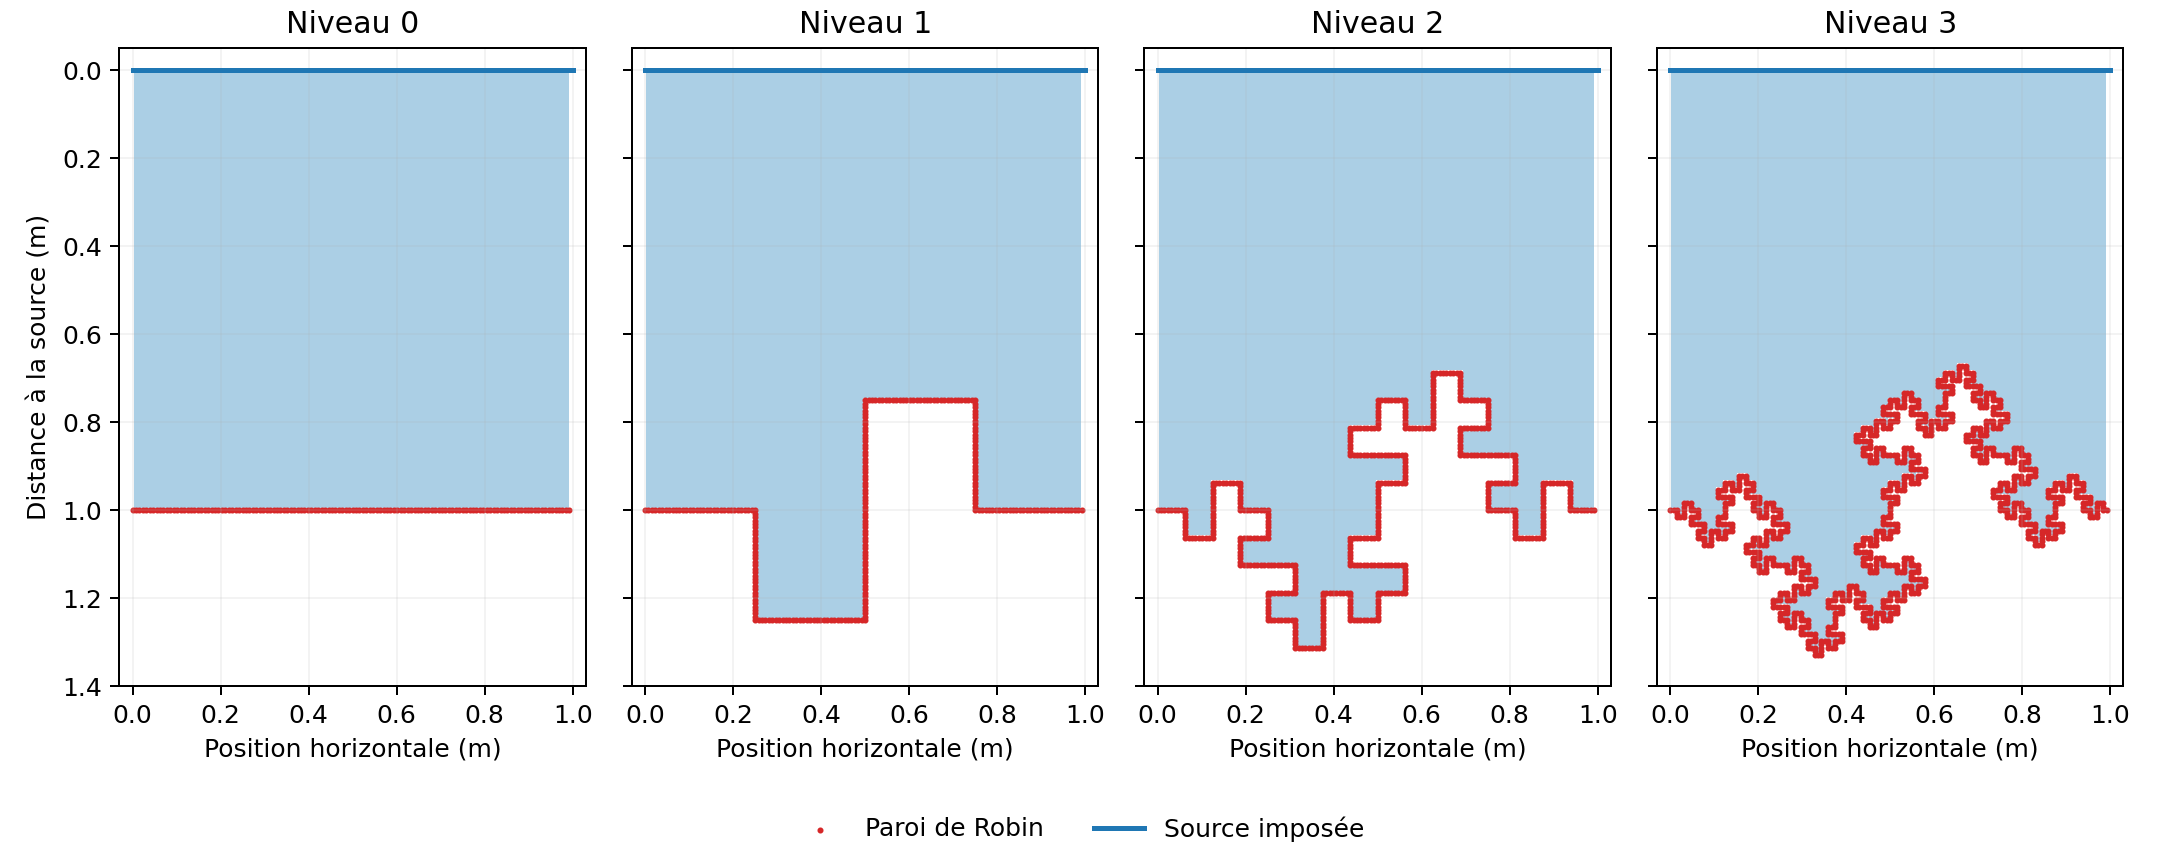
\includegraphics[width=.94\textwidth,height=.30\textheight,keepaspectratio]{fig_geometries.png}
\caption{Domaines d’air et contours aux quatre niveaux}
\label{fig:geometries}
\end{figure}

La construction nominale conserve une aire de $1\,\mathrm{m^2}$. La longueur du mur double à chaque niveau, tandis que le plus petit segment est divisé par quatre. Le tableau~\ref{tab:geometries} distingue ces valeurs géométriques des points utilisés par la quadrature du code.
\begin{table}[!htbp]
\centering\small
\begin{tabular}{crrrr}
\toprule
Niveau & Longueur nominale (m) & Points Robin & Pas par petit segment & $h^2\#\Omega_h$ ($\mathrm{m^2}$)\\
\midrule
0 & 1 & 128 & 128 & 0,976685\\
1 & 2 & 256 & 32 & 0,972778\\
2 & 4 & 512 & 8 & 0,964966\\
3 & 8 & 1\,024 & 2 & 0,949341\\
\bottomrule
\end{tabular}
\caption{Géométrie nominale et représentation sur la grille}
\label{tab:geometries}
\end{table}
La longueur d'onde $\lambda=c/f$ fournit aussi un repère pour la taille des irrégularités. Une longueur de $0,25$ m est égale à $\lambda/2$ vers 686 Hz, et une longueur de $0,0625$ m vers 2\,744 Hz. Ces ordres de grandeur relient les niveaux un et deux à la bande choisie. Ils servent de repères d'échelle, puis l'effet réel des motifs est mesuré sur les spectres.

La grille de stockage comporte $256\times128$ points et son pas vaut $h=1/128$ m. Les points de bord et les points extérieurs sont exclus de la somme dans l'air, d'où une aire de quadrature légèrement différente de l'aire nominale du polygone. Les coordonnées horizontales stockées vont de zéro à $0,9921875$ m. Le contour de niveau deux s'étend entre les ordonnées $0,6875$ et $1,3125$ m. Ces dimensions définissent notre modèle réduit.
\section{Modélisation de la source acoustique du RER B}
\subsection{Une excitation uniforme sur le bord supérieur}
Les fonctions \code{source_constant(y, omega)} et \code{source_rer_b(y, omega)} définissent l'excitation. L'argument $y$ désigne la position le long du bord supérieur et $\omega$ la pulsation. Les deux sources proposées sont indépendantes de $y$, donc elles imposent une amplitude et une phase uniformes sur ce bord. La première renvoie un, alors que la seconde suit le spectre défini ci-dessous. Le paramètre \code{SOURCE}, placé au début de \code{demo_control_polycopie2024.py}, choisit la fonction utilisée pour l'identification du coefficient, le champ initial, la descente et la courbe fréquentielle.

Cette hypothèse est une simplification du cas d'usage. Le mouvement d'un train ne suffit pas à rendre sa pression uniforme. Des profils uniforme, localisé et oblique sont ensuite comparés en conservant la même somme des amplitudes au carré sur le bord d'entrée.

\subsection{Somme de trois composantes gaussiennes}
La fonction \code{source_rer_b}, dans \code{preprocessing.py}, convertit la pulsation en fréquence par $f=\omega/(2\pi)$, puis fournit l'amplitude relative
\begin{equation}\label{eq:source}
G(f)=\sum_{m=1}^{3}A_m\exp\!\left(-\frac{(f-f_m)^2}{2\sigma_m^2}\right)
\end{equation}
Le centre $f_m$ et l'écart-type $\sigma_m$ sont exprimés en hertz. L'écart-type règle la largeur de la composante et $A_m$ son amplitude maximale lorsqu'elle est considérée seule. L'argument $y$ est conservé dans la signature pour que les deux sources aient la même forme d'appel. Les neuf paramètres retenus dans \eqref{eq:source} figurent dans le tableau~\ref{tab:source}.

\begin{table}[htbp]
\centering
\begin{tabular}{p{6.1cm}rrr}
\toprule
Composante & $f_m$ (Hz) & $\sigma_m$ (Hz) & $A_m$\\
\midrule
Basses fréquences, traction et équipements & 200 & 100 & 1,0\\
Roulement & 800 & 350 & 0,8\\
Haute fréquence, crissement représentatif & 2\,500 & 150 & 0,5\\
\bottomrule
\end{tabular}
\caption{Paramètres du spectre hypothétique de la source}
\label{tab:source}
\end{table}

Le centre de 200 Hz s'appuie sur les contributions basses fréquences observées à l'intérieur du RER B par Lee et ses coauteurs \cite{lee2022}. Il regroupe plusieurs mécanismes et n'est pas attribué exclusivement aux moteurs. Le centre de 800 Hz reprend un ordre de grandeur observé pour le bruit roue--rail sur d'autres métros \cite{metro2026}.

La composante à 2\,500 Hz sert à représenter une contribution haute fréquence plus étroite. Cette fréquence apparaît dans des observations roue--rail \cite{metro2026}, tandis que les mesures de crissement font apparaître différents pics suivant les conditions de contact \cite{kim2019}. L'association exacte du crissement à 2\,500 Hz reste donc un choix de l'étude.

Les écarts-types et les amplitudes relatives sont également choisis pour cette première représentation. Le modèle n'a pas été ajusté à un enregistrement extérieur du RER B. La gaussienne de roulement est large et la troisième plus resserrée, afin de distinguer une contribution étendue d'une contribution davantage tonale. La somme décrit une enveloppe d'amplitude, et sa valeur totale peut dépasser l'amplitude de chacune des composantes.

La figure~\ref{fig:source} montre cette enveloppe d'amplitude. La zone grisée repère la bande de 50 à 3\,500 Hz résolue par le programme. Les deux premières composantes se recouvrent et la contribution haute fréquence est plus resserrée.
\begin{figure}[!htbp]
\centering
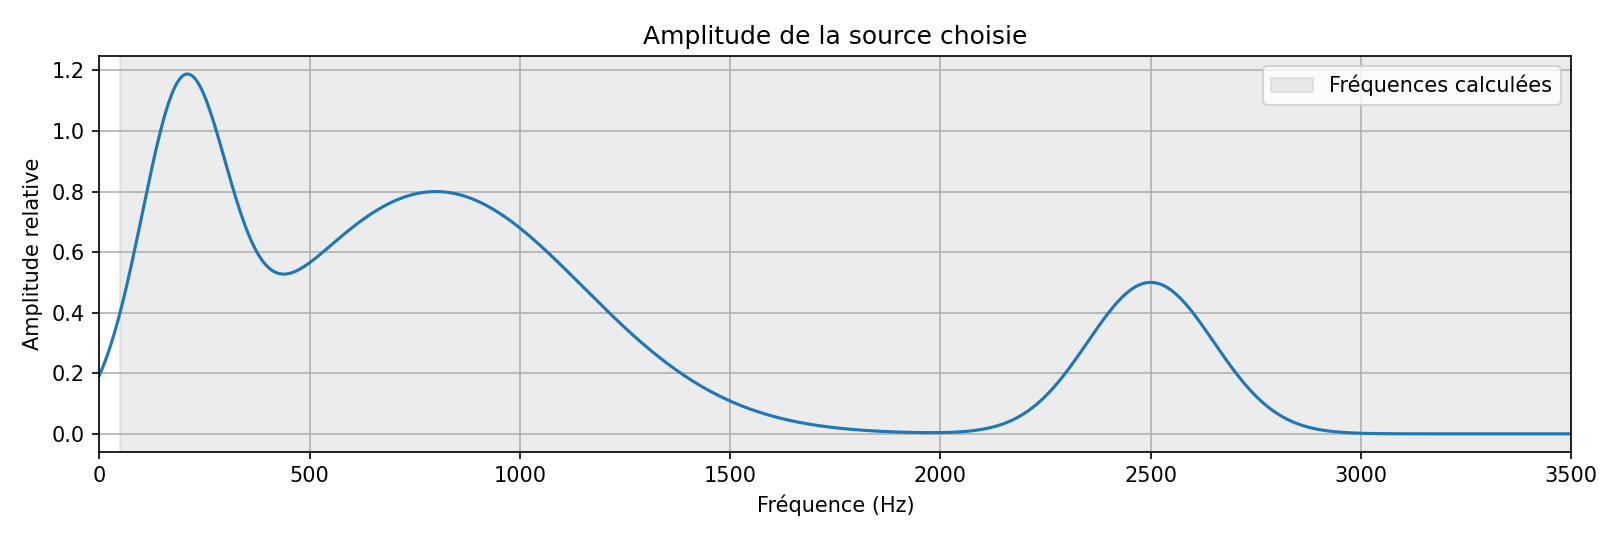
\includegraphics[width=.94\textwidth,height=.25\textheight,keepaspectratio]{fig_rer_b_spectre.png}
\caption{Amplitude de la source en fonction de la fréquence}
\label{fig:source}
\end{figure}

\subsection{Portée de la pondération fréquentielle}
Pour une géométrie et une répartition fixées, la linéarité de Helmholtz donne, lorsque les autres sources sont nulles,
\begin{equation*}
u_f=G(f)u_f^{(1)}\qquad J(f)=|G(f)|^2J^{(1)}(f)
\end{equation*}
L'exposant $(1)$ désigne le calcul avec une source unitaire. À une fréquence fixée et pour $G(f)\ne0$, ce facteur conserve le classement des panneaux. Sur une bande, il donne davantage d'importance à certaines fréquences et peut modifier le meilleur compromis. Une baisse de l'énergie due seulement à une source moins forte ne démontre donc pas une amélioration du mur.

Les amplitudes restent relatives. Elles ne permettent pas de déduire directement un niveau absolu en dB(A), qui demanderait une référence de pression, une calibration et une pondération acoustique adaptées.

\section{Matériaux poreux et coefficient de paroi}
\subsection{Matériaux comparés}
Les caractéristiques du dictionnaire \code{MATERIAUX} sont la porosité $\phi$, la tortuosité $\alpha_h$ et la résistivité au passage de l'air $\sigma$. La porosité mesure la fraction du volume occupée par les pores, la tortuosité décrit l'allongement des trajets dans les pores et la résistivité traduit la résistance à l'écoulement. Le tableau~\ref{tab:materiaux} contient les trois matériaux effectivement comparés.
\begin{table}[!htbp]
\centering
\begin{tabular}{lrrr}
\toprule
Matériau & $\phi$ & $\alpha_h$ & $\sigma$ ($\mathrm{Pa\,s\,m^{-2}}$)\\
\midrule
Laine de roche & 0,97 & 1,10 & 30\,000\\
Mélamine & 0,99 & 1,02 & 14\,000\\
Laine de verre & 0,99 & 1,10 & 20\,000\\
\bottomrule
\end{tabular}
\caption{Caractéristiques des matériaux comparés}
\label{tab:materiaux}
\end{table}
La laine de roche sert de matériau de référence pour les études de placement. La comparaison finale utilise les trois matériaux avec la même source, les mêmes fréquences et le budget de matériau annoncé.

\subsection{Identification du coefficient complexe}
La fonction \code{materiau} transforme les caractéristiques précédentes en coefficients du modèle poreux. \code{compute_alpha} applique ensuite l'identification du §3.2.4 du polycopié \cite{cours}. Elle compare le champ d'un modèle avec pertes dans le volume du matériau et celui d'un modèle équivalent avec une condition de Robin. Les poids $A=B=1$ portent sur les différences des champs et de leurs gradients. La fonction \code{scipy.optimize.minimize} ajuste les parties réelle et imaginaire d'alpha par la méthode de Nelder--Mead, qui déplace des couples d'essai pour réduire cette erreur.

Avec les notations du modèle poreux, les coefficients sont
\begin{equation*}
\eta_1=\frac{\phi}{\alpha_h}
\qquad
 a=\frac{\sigma\phi^2\gamma_p}{c_0^2\rho_0\alpha_h}
\qquad
\xi_1=\frac{\phi\gamma_p}{c_0^2}
\end{equation*}
Le coefficient $a$ décrit les pertes dans le matériau. \code{g_k} calcule les coefficients de Fourier de la source sur le bord auxiliaire. Pour l'indice entier $n$, le nombre d'onde transversal est $k_n=n\pi/l$, et
\begin{equation*}
g_n(\omega)=\frac{1}{2l}\int_{-l}^{l}g(y,\omega)e^{-\ii k_ny}\dd y
\end{equation*}
Les fonctions \code{lambda0} et \code{lambda1} décrivent ensuite la propagation de ces composantes dans l'air et le matériau. \code{erreur} additionne les erreurs modales pour évaluer la différence des deux champs et de leurs gradients. L'identification minimise ainsi une erreur du type
\begin{equation*}
E(\alpha)=A\|u_{\mathrm{volume}}-u_{\mathrm{Robin}}(\alpha)\|_{L^2}^2
+B\|\nabla u_{\mathrm{volume}}-\nabla u_{\mathrm{Robin}}(\alpha)\|_{L^2}^2
\end{equation*}
Les normes sont prises dans la partie air du domaine auxiliaire. La comparaison concerne le même matériau et la même excitation, avec deux représentations différentes de ses pertes.

Le domaine auxiliaire a pour demi-largeur $l=2,5$ m et pour longueur $L=10$ m. Le paramètre $\Delta x_\alpha=0,5$ m fixe $N_\alpha=L/\Delta x_\alpha=20$, donc 41 modes de Fourier d'indices $-20$ à 20. On utilise $\rho_0=1,2\,\mathrm{kg\,m^{-3}}$, $c_0=343\,\mathrm{m\,s^{-1}}$, $\gamma_p=1,4$, $\eta_0=1$ et $\xi_0=c_0^{-2}$. Ces longueurs et ces modes appartiennent au problème d'identification, indépendamment de la grille de propagation.

Le point initial est \code{ALPHA0=[50, -50]}, et les tolérances \code{xatol} et \code{fatol} valent $10^{-6}$ et $10^{-10}$. L'indicateur \code{success} est vérifié avant d'utiliser le coefficient. \code{compute_material_coefficients} répète ce calcul aux 70 fréquences. Le coefficient est gardé fixe pendant une descente à une fréquence et recalculé lorsque la fréquence change.

La figure~\ref{fig:materiaux} présente les parties réelle et imaginaire obtenues par \code{study_porous_materials}. Les signes respectent la convention du modèle. Pour la laine de roche à $\omega_0=3\,430\,\mathrm{rad\,s^{-1}}$, on obtient $\alpha=18,154584-21,197637\ii\,\mathrm{m^{-1}}$. À 50, 2\,500 et 3\,500 Hz, on trouve respectivement $5,894818-5,979421\ii$, $30,137224-58,478507\ii$ et $31,996643-77,112209\ii$, en $\mathrm{m^{-1}}$.

\begin{figure}[!htbp]
\centering
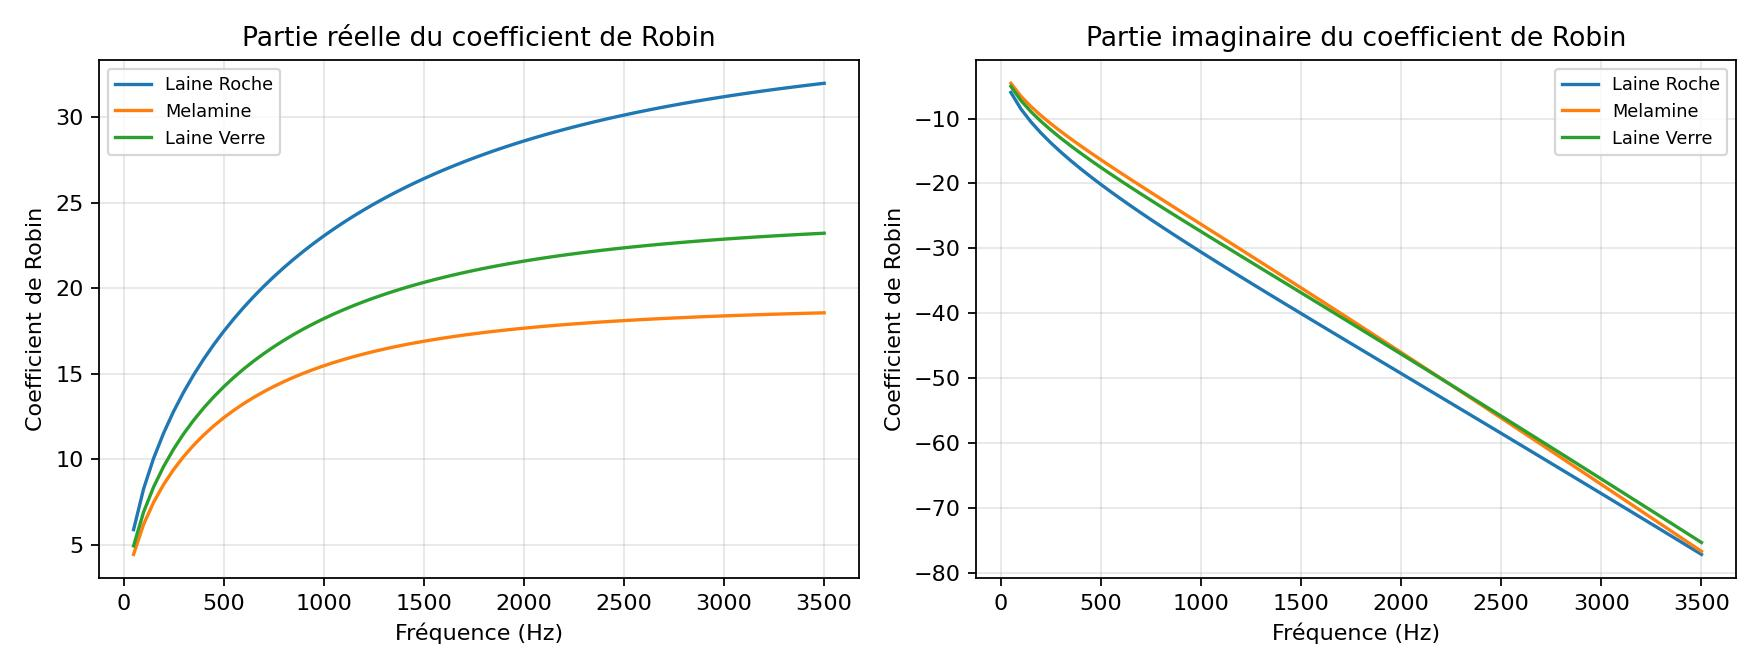
\includegraphics[width=.94\textwidth,height=.29\textheight,keepaspectratio]{resultats_materiaux_validation/fig_comparaison_materiaux.jpg}
\caption{Parties réelle et imaginaire du coefficient des trois matériaux}
\label{fig:materiaux}
\end{figure}

Les trois matériaux donnent des coefficients différents, mais la seule taille d'alpha ne suffit pas à les classer. Le critère dépend aussi de la forme, du placement et de la fréquence. Leur classement est donc établi en résolvant le problème acoustique pour chacun d'eux.
\section{Discrétisation et problème d’optimisation}
\subsection{Assemblage et résolution}
Le stencil à cinq points utilise un point et ses quatre voisins pour approcher le Laplacien
\begin{equation*}
\Delta u_{i,j}\simeq\frac{u_{i+1,j}+u_{i-1,j}+u_{i,j+1}+u_{i,j-1}-4u_{i,j}}{h^2}
\end{equation*}
Les fonctions \code{compute_stiffness_matrix} et \code{compute_mass_matrix} construisent les contributions spatiales et celles du terme $k_f^2u_f$. Les fonctions \code{compute_dirichlet_condition}, \code{compute_neumann_condition} et \code{compute_robin_condition} ajoutent les données de bord. \code{solve_helmholtz} résout le système linéaire obtenu. Pour les coefficients unitaires et une donnée de Robin nulle, la valeur du point de bord $u_B$ est reliée à celle du voisin intérieur $u_I$ par
\begin{equation*}
u_B=\frac{u_I}{1+h\alpha\chi_B}
\end{equation*}
Le paramètre nommé \code{omega} par le solveur historique reçoit le nombre d'onde $k_f=\omega/c$. L'identification \code{compute_alpha} et les fonctions de source reçoivent la pulsation temporelle $\omega=2\pi f$.

La classe \code{FastHelmholtzSolver} conserve les contributions fixes de la grille pour les résolutions répétées et travaille sur les inconnues intérieures. Cette classe réutilise la même factorisation pour le champ et pour l'adjoint, dont le système fait intervenir la transposée conjuguée de la matrice. Les champs enregistrés valent zéro sur les points non intérieurs car ces valeurs ne sont pas reconstruites par le solveur. Les cartes les masquent pour représenter uniquement l'air calculé.

\subsection{Critères à une fréquence et sur une bande}
Pour une forme et une source fixées, le critère du §7.4.2 du cours \cite{cours} est
\begin{equation*}
J(f,\chi)=\int_\Omega|u_f(x;\chi)|^2\dd x
\qquad
J_h(f,\chi)=h^2\sum_{(i,j)\in\Omega_h}|u_{i,j}|^2
\end{equation*}
$\Omega_h$ est l'ensemble des points intérieurs. Le module au carré mesure l'amplitude de pression au carré, donc un coût plus faible correspond à un champ globalement moins intense pour les mêmes données. \code{your_compute_objective_function} et \code{FastHelmholtzSolver.compute_energy} calculent cette somme. Sa valeur est une amplitude relative au carré multipliée par une aire.

Le coût intégré sur la bande et sa moyenne sont calculés par la règle des trapèzes, avec $F=70$ fréquences \cite{cours}
\begin{equation*}
\mathcal J_h=\sum_{r=1}^{F-1}\frac{f_{r+1}-f_r}{2}
\left[J_h(f_r,\chi)+J_h(f_{r+1},\chi)\right]
\qquad
\overline J_h=\frac{\mathcal J_h}{f_F-f_1}
\end{equation*}
La fonction \code{mean_cost} fournit cette moyenne. Le facteur spectral de la source est déjà appliqué au champ, donc les coûts sont intégrés directement. Ces indicateurs permettent une comparaison relative du modèle.

\subsection{Quantité imposée et valeurs intermédiaires}
Dans le problème continu, une fraction $\beta$ de mur garnie impose $\int_{\Gamma_R}\chi\dd s=\beta|\Gamma_R|$, avec $|\Gamma_R|$ la longueur du mur. Le cours recherche d'abord un minimum avec $0\leq\chi\leq1$, puis construit une répartition binaire \cite{cours}. Autoriser les valeurs intermédiaires rend possible une recherche progressive. Le résultat d'existence du §7.4.3 concerne ce problème continu avec valeurs intermédiaires.

L'ensemble des densités autorisées à fraction $\beta$ s'écrit
\begin{equation*}
\mathcal U(\beta)=\left\{\chi:\Gamma_R\longrightarrow[0,1]\,\middle|\,
\int_{\Gamma_R}\chi\dd s=\beta|\Gamma_R|\right\}
\qquad
\min_{\chi\in\mathcal U(\beta)}J(f,\chi)
\end{equation*}
Pour la recherche de forme, on compare les minima numériques trouvés pour un catalogue de contours. Le programme conserve la forme pendant chaque descente et modifie la répartition $\chi$.

Le code utilise une contrainte sur les $S$ points de Robin. La fonction \code{project_density} impose
\begin{equation*}
0\leq\chi_j\leq1
\qquad \sum_{j=1}^{S}\chi_j=V_{\mathrm{obj}}S
\end{equation*}
Les historiques et les spectres complets sont conservés dans les fichiers CSV, NPZ et JSON associés.

Le paramètre \code{V_obj} est une fraction nodale. À la fin, \code{binarize_chi} conserve les $q=\operatorname{round}(V_{\mathrm{obj}}S)$ valeurs les plus grandes et les met à un, puis met les autres à zéro. L'arrondi peut modifier la quantité continue d'un demi-point au plus.

Sur un même mur, cette contrainte compare des placements à quantité fixée. Entre formes différentes, on ajoute un budget commun de $q=38$ points garnis, obtenu à partir de $\operatorname{round}(0,30\times128)$. La fraction est alors $q/S$ pour chaque forme. On définit le budget discret pondéré par le pas
\begin{equation}\label{eq:budget}
Q_h=h\sum_{j=1}^{S}\chi_j=\frac{38}{128}=0,296875\,\mathrm{m}
\end{equation}
Ce budget nodal est une approximation pour comparer les calculs sur une même grille. Il doit être distingué de la longueur exacte d'une portion garnie du polygone, notamment aux coins et aux points du bord qui ne sont pas adjacents à un point intérieur. L'argument \code{fixed_covered_nodes} de \code{compare_absorber_configurations} rend ce choix explicite.

\subsection{Adjoint et gradient}
Le gradient mesure l'effet d'une petite modification de chaque densité sur le coût. Le §7.5.2 introduit un problème adjoint pour le calculer sans résoudre un problème différent pour chaque point du mur \cite{cours}. On applique ce principe au système assemblé
\begin{equation*}
A(\chi)U=b(\chi)
\qquad J_h=U^*WU
\qquad A^*P=2WU
\end{equation*}
$U$ est le vecteur du champ complexe, $b$ le second membre et $P$ l'adjoint. L'étoile désigne la transposée conjuguée. La matrice diagonale $W$ vaut $h^2$ aux points intérieurs et zéro ailleurs. Pour une variation réelle de $\chi_j$, la composante du gradient est
\begin{equation*}
g_j=\operatorname{Re}\!\left[P^*\left(\frac{\partial b}{\partial\chi_j}
-\frac{\partial A}{\partial\chi_j}U\right)\right]
\end{equation*}
Les fonctions \code{compute_state}, \code{compute_adjoint} et \code{compute_gradient} réalisent ces étapes. Dans les études, la source reste fixe et le second membre Robin est nul. Le terme $\partial b/\partial\chi_j$ est alors nul. La classe \code{FastHelmholtzSolver} calcule le même gradient pour le système réduit aux points intérieurs.

\subsection{Descente projetée et passage binaire}
La descente du §7.6 fait un pas dans la direction opposée au gradient, puis ramène la proposition dans l'ensemble des densités autorisées \cite{cours}. La projection s'écrit
\begin{equation*}
\chi_j^{n+1}=\max\!\left(0,\min\!\left(\chi_j^n-\mu_ng_j^n+\ell_n,1\right)\right)
\end{equation*}
Le pas est $\mu_n$ et $\ell_n$ est un décalage commun qui conserve la somme des densités. \code{project_density} le cherche par 60 étapes de dichotomie, c'est-à-dire en divisant successivement un intervalle de recherche en deux. Le pas initial vaut 5. Une proposition est acceptée si le coût diminue strictement, puis le pas est multiplié par $1,1$. Sinon, il est divisé par deux.

Les études comparatives utilisent au plus 80 itérations. L'arrêt se fait aussi si le pas devient inférieur ou égal à $10^{-5}$ ou si la plus grande variation acceptée de densité devient inférieure à $10^{-7}$. La démonstration initiale conserve les 100 itérations du programme fourni, dans \code{your_optimization_procedure}.

\code{optimize_single_frequency} renvoie une répartition continue et son historique. Le passage binaire est ensuite mesuré séparément en recalculant le champ et son coût. Cette opération peut augmenter ou diminuer le coût, donc la décroissance observée pendant la descente concerne les étapes continues acceptées.

\subsection{Critère multifréquence et choix des cibles}
La fonction \code{optimize_multi_frequency} recherche une seule répartition pour plusieurs fréquences. Si $m$ fréquences $f_r$ sont retenues, avec des poids $w_r$ positifs de somme un, le coût est
\begin{equation}\label{eq:multi}
J_{\mathrm{cibles}}(\chi)=\sum_{r=1}^{m}w_rJ_h(f_r,\chi)
\end{equation}
Les études utilisent les mêmes poids $w_r=1/m$, avec au plus trois cibles. Les gradients sont additionnés avec ces poids. Ce critère est une moyenne sur les cibles, distincte de $\overline J_h$ calculé sur toute la bande. L'évaluation des 70 fréquences après optimisation vérifie donc aussi les effets entre les cibles.

La fonction \code{find_local_maxima} repère les valeurs plus grandes que leurs voisines. Un pic est retenu si sa hauteur par rapport aux minima voisins atteint au moins $1\,\%$ de l'étendue du spectre. Le voisinage couvre jusqu'à six échantillons de chaque côté, soit 300 Hz. \code{select_peak_indices} classe ces pics par coût et complète avec les plus grandes valeurs échantillonnées si nécessaire. Deux cibles sont retenues par forme pour le placement monofréquence et trois pour le placement multifréquence.

\subsection{Paramètres des études et résolution spatiale}
Les calculs principaux sont faits avec $N=128$, $M=256$ et $h=1/128$ m. La bande va de 50 à 3\,500 Hz par pas de 50 Hz, soit 70 fréquences. On utilise la source RER et la laine de roche pour le placement. La fraction principale vaut $0,30$, donc les placements binaires comptent 38, 77 et 154 points garnis aux niveaux zéro, un et deux. Les fractions testées pour la quantité sont $0,10$, $0,30$, $0,50$, $0,70$ et un. Le cas initial séparé utilise $\omega_0=3\,430\,\mathrm{rad\,s^{-1}}$, donc $k_0=10\,\mathrm{m^{-1}}$ et $f_0\simeq545,90$ Hz, avec 204 points garnis sur 512.

À 3\,500 Hz, la longueur d'onde $\lambda=c/f$ comporte $\lambda/h=12,544$ pas de grille, ce qui satisfait la règle des dix points par longueur d'onde. Le §7.7 demande aussi dix points dans les portions garnies et nues \cite{cours}. Le tri point par point peut créer des portions d'un point et n'impose donc pas cette dernière condition. De même, le niveau trois ne contient que deux pas par petit segment. Il est présenté comme une exploration sur cette grille. Le pas fréquentiel de 50 Hz repère des maxima échantillonnés et peut manquer des pics plus étroits.
\section{Vérifications du modèle et du calcul}
\subsection{Paroi ouverte et paroi réfléchissante}
La fonction \code{study_sommerfeld_open_air_vs_reflexive} compare une paroi réfléchissante, une sortie ouverte et une paroi entièrement garnie de laine de roche. Pour la sortie ouverte, la condition de Sommerfeld est $\partial_nu_f-\ii k_fu_f=0$. Dans notre convention, son coefficient vaut donc $\alpha=-\ii k_f$.

On considère un rectangle de largeur $w$ et de profondeur $d$, avec une source uniforme $G(f)$ à l'entrée. Si $s$ est la distance à cette entrée, la solution de Helmholtz est
\begin{equation*}
u_{\mathrm{ouv}}(s)=G(f)e^{\ii k_fs}
\qquad
u_{\mathrm{refl}}(s)=G(f)\frac{\cos(k_f(d-s))}{\cos(k_fd)}
\end{equation*}
La deuxième expression est définie pour $\cos(k_fd)\ne0$. En intégrant le module au carré, on obtient la dépendance à la profondeur de cette famille de formes
\begin{equation*}
J_{\mathrm{ouv}}(d)=w|G(f)|^2d
\qquad
J_{\mathrm{refl}}(d)=w|G(f)|^2\frac{d/2+\sin(2k_fd)/(4k_f)}{\cos^2(k_fd)}
\end{equation*}
À fréquence fixée, la première quantité croît linéairement avec la profondeur. La seconde varie fortement lorsque $\cos(k_fd)$ se rapproche de zéro, car les réflexions produisent une onde stationnaire. Ces expressions résultent de l'application de Helmholtz au rectangle uniforme. La fonction Python les évalue pour $w=d=1$.

La figure~\ref{fig:parois} confronte ces références continues aux coûts discrets. Les coûts moyens de bande valent \BoundaryReflectingCost{} pour la paroi réfléchissante, \BoundaryOpenCost{} pour la sortie ouverte et \BoundaryMaterialCost{} pour la laine de roche. L'écart relatif entre les courbes ouverte discrète et continue vaut \BoundaryOpenError\,\%. La sortie ouverte supprime le retour idéal de l'onde, alors que la paroi poreuse laisse subsister une réponse dépendante de la fréquence. L'écart annoncé est la norme euclidienne de la différence des 70 coûts, divisée par la norme des 70 coûts de la référence continue.

\begin{figure}[!htbp]
\centering
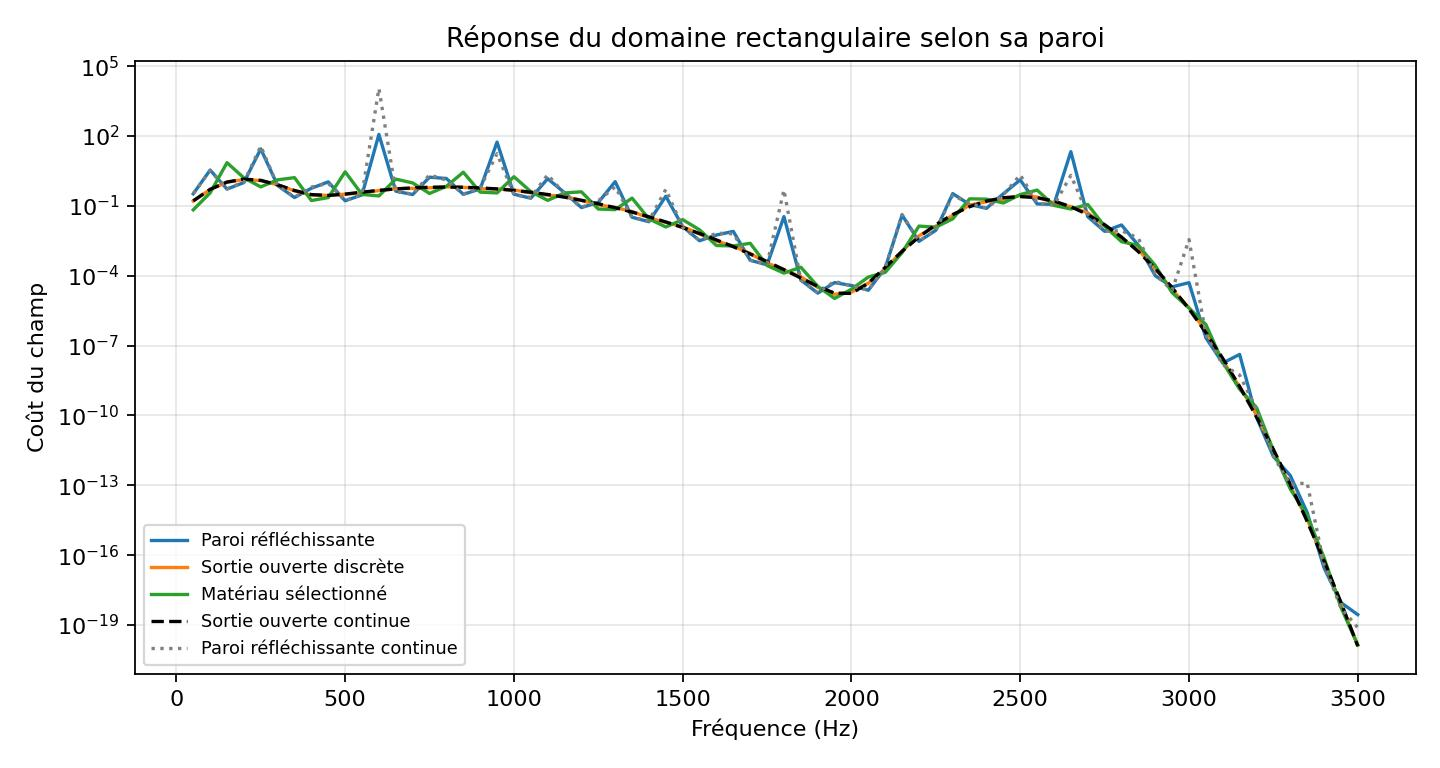
\includegraphics[width=.94\textwidth,height=.36\textheight,keepaspectratio]{resultats_materiaux_validation/fig_sommerfeld_vs_reflexif.jpg}
\caption{Coût du champ selon la fréquence et la condition de paroi}
\label{fig:parois}
\end{figure}

Pour comparer des formes de même aire $A_\Omega=1\,\mathrm{m^2}$, on pose $w=A_\Omega/d$. Le coût ouvert vaut alors $A_\Omega|G(f)|^2$ et le coût réfléchi conserve sa dépendance à la profondeur. En dérivant les expressions précédentes à fréquence fixée, on obtient
\begin{equation*}
\frac{\partial J_{\mathrm{ouv}}}{\partial d}=0
\qquad
\frac{\partial J_{\mathrm{refl}}}{\partial d}
=\frac{A_\Omega|G(f)|^2-J_{\mathrm{refl}}(d)}{d}
+2k_fJ_{\mathrm{refl}}(d)\tan(k_fd)
\end{equation*}
La figure~\ref{fig:profondeur} représente ce calcul à 200 Hz pour 201 profondeurs entre $0,5$ et $1,5$ m, avec une largeur $w=A_\Omega/d$. \code{study_boundary_depth_dependence} évalue les solutions continues sur cette famille de rectangles. La réponse réfléchissante dépend fortement de la forme près des résonances, là où le coût ouvert conserve ici la valeur $A_\Omega|G(f)|^2$ à aire fixée.
\begin{figure}[!htbp]
\centering
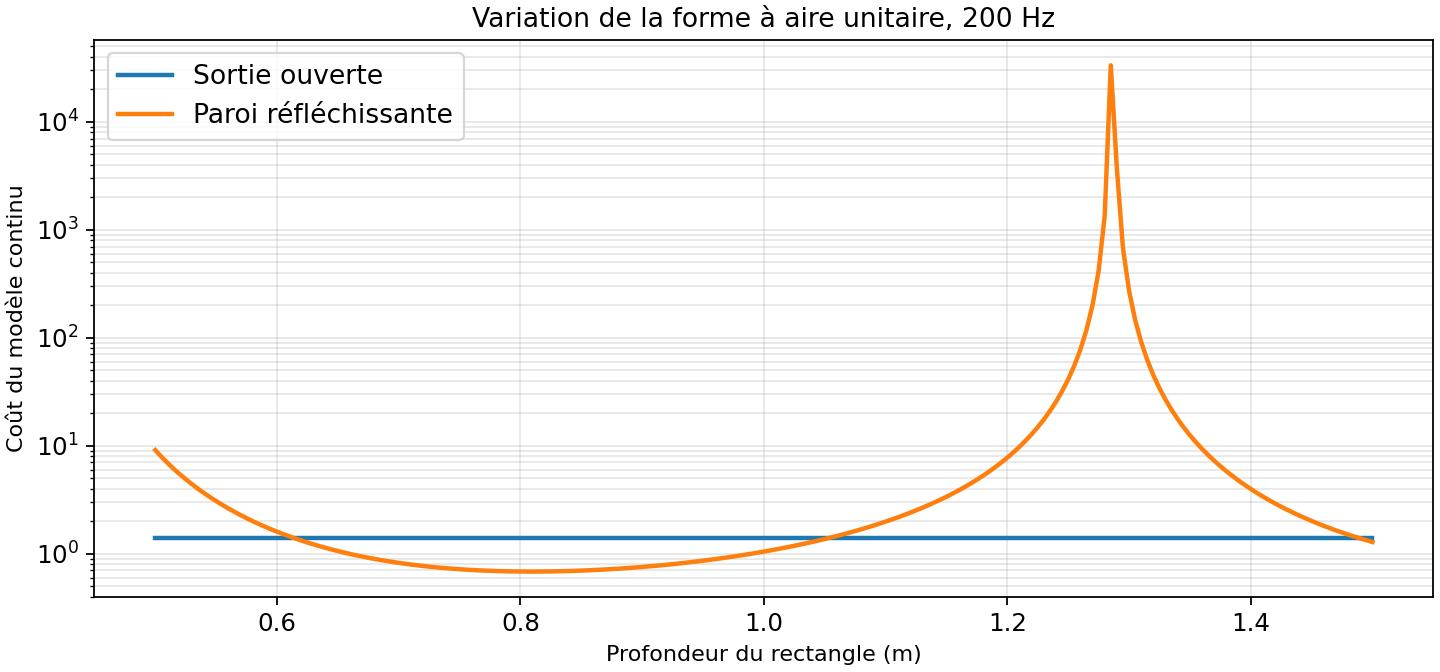
\includegraphics[width=.90\textwidth,height=.30\textheight,keepaspectratio]{resultats_materiaux_validation/fig_cout_profondeur_rectangle.jpg}
\caption{Coût continu en fonction de la profondeur à aire constante}
\label{fig:profondeur}
\end{figure}

\subsection{Vérification du gradient}
\code{validate_adjoint_gradient} compare la dérivée adjointe à la variation du coût après une petite perturbation positive puis négative d'une densité. Le contrôle porte sur 12 points répartis le long du mur, avec un pas de perturbation de $10^{-6}$, au niveau un et à $\omega_0=3\,430\,\mathrm{rad\,s^{-1}}$. La figure~\ref{fig:gradient} montre la superposition des dérivées. L'erreur relative, calculée par la norme des différences divisée par la norme des dérivées obtenues par perturbation, vaut $\GradientRelativeError$.

\begin{figure}[!htbp]
\centering
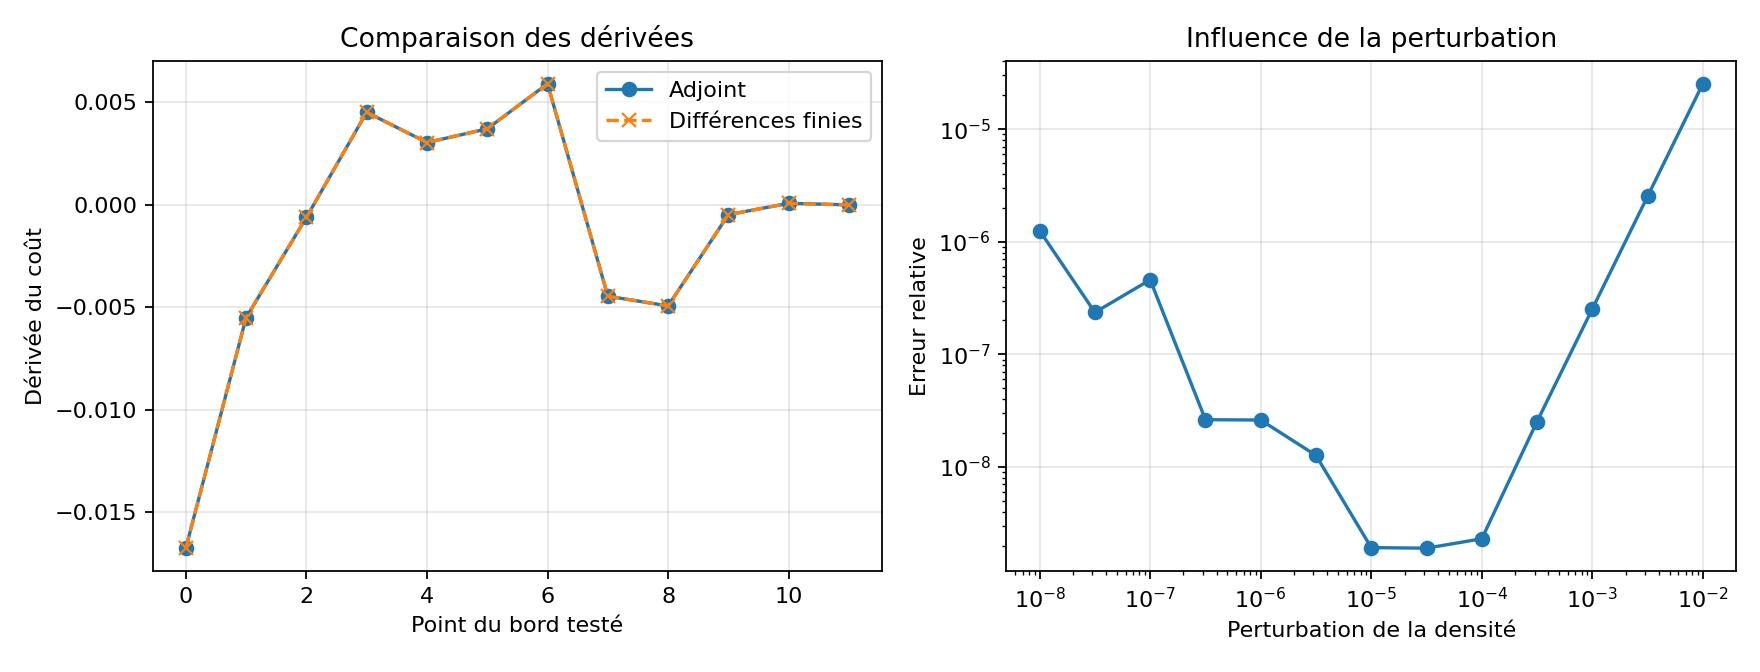
\includegraphics[width=.94\textwidth,height=.28\textheight,keepaspectratio]{resultats_materiaux_validation/fig_validation_gradient_adjoint.jpg}
\caption{Dérivée adjointe et différences centrées du coût}
\label{fig:gradient}
\end{figure}

Une seconde courbe fait varier la perturbation entre $10^{-8}$ et $10^{-2}$ sur 13 valeurs. Aux plus petites perturbations, la soustraction de deux coûts proches amplifie l'effet des erreurs d'arrondi. Aux plus grandes, la variation n'est plus suffisamment petite pour approcher la dérivée locale avec la même précision. La zone intermédiaire confirme l'accord entre les deux calculs.

\subsection{Premier essai à une fréquence}
Le cas de démonstration utilise le niveau deux et 204 points garnis sur 512, soit $V_{\mathrm{obj}}=0,398438$. À $\omega_0=3\,430\,\mathrm{rad\,s^{-1}}$, l'amplitude de source vaut $0,617187$. La figure~\ref{fig:demo} reprend ce premier calcul de \code{your_optimization_procedure} avec la même loi de laine de roche.

\begin{figure}[!htbp]
\centering
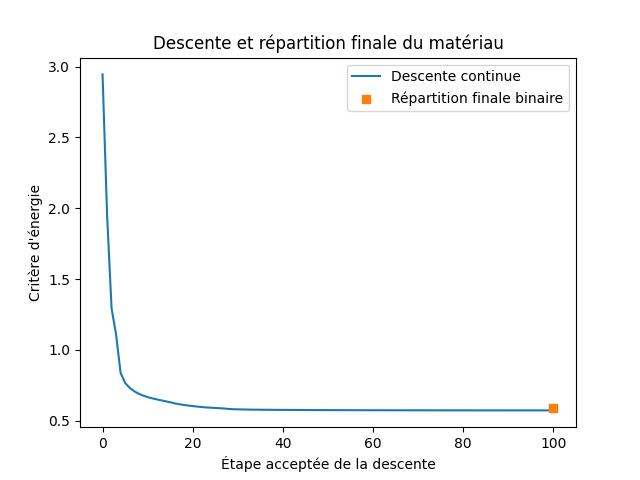
\includegraphics[width=.80\textwidth,height=.29\textheight,keepaspectratio]{fig_energy_real.jpg}
\caption{Coût de la démonstration pendant la descente et après tri binaire}
\label{fig:demo}
\end{figure}

Le coût initial passe de $1,126340$ à $0,223515$ après 100 étapes continues acceptées. Le coût recalculé pour le placement binaire vaut $0,223519$, avec 204 points garnis. Ce cas vérifie la chaîne source--champ--adjoint--gradient--projection. Les comparaisons suivantes utilisent une fraction de $0,30$ et au plus 80 itérations, donc leurs chiffres ne doivent pas être confondus avec cet essai initial.
La figure~\ref{fig:premierebande} donne également le coût sur la bande pour cette répartition initiale de 204 points garnis. \code{run_rer_b_frequency_sweep} réévalue la source et le coefficient à chaque fréquence. Le maximum échantillonné vaut $10,8487$ à 400 Hz et le coût intégré vaut $4\,416,119652$. Cette courbe de référence utilise une quantité différente de celle des études comparatives à fraction $0,30$.
\begin{figure}[!htbp]
\centering
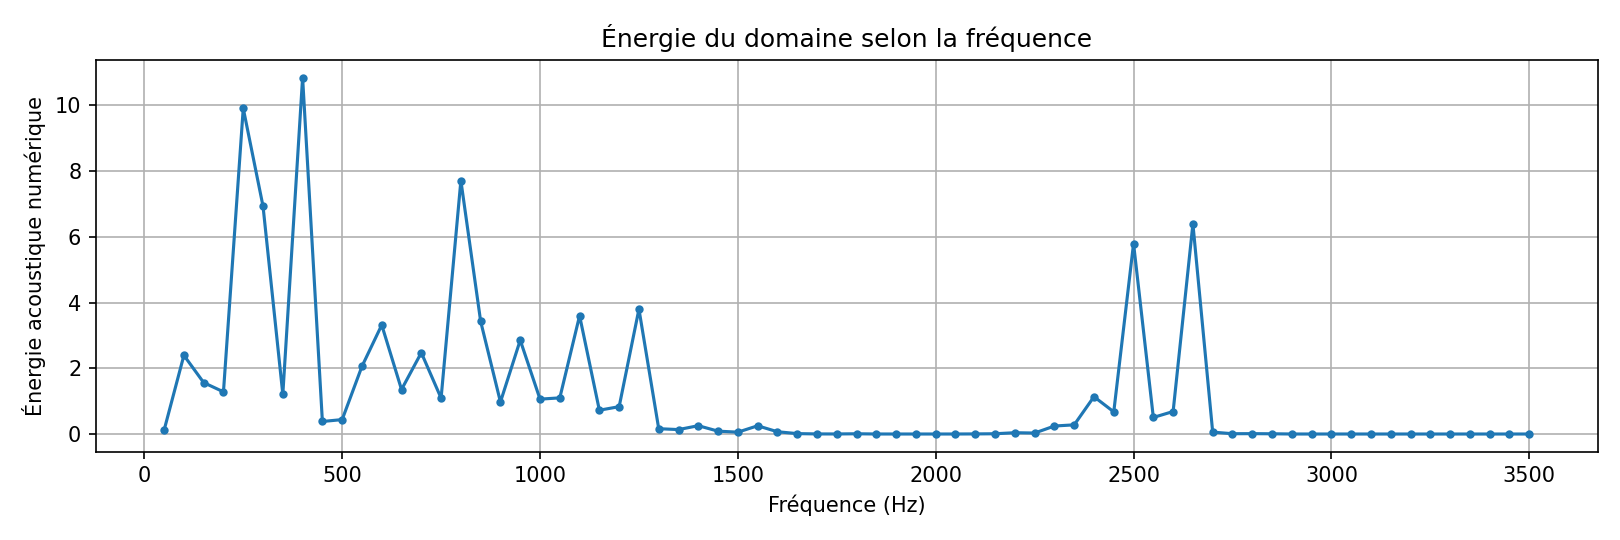
\includegraphics[width=.94\textwidth,height=.25\textheight,keepaspectratio]{fig_rer_b_energie.png}
\caption{Coût fréquentiel de la répartition initiale à 204 points garnis}
\label{fig:premierebande}
\end{figure}

\section{Spectres des murs et placement monofréquence}
\subsection{Mur plan entièrement garni et maxima}
La fonction \code{study_spectra_and_single_frequency_placement} calcule d'abord le coût sur les 70 fréquences pour un mur entièrement garni. La figure~\ref{fig:murplan} montre le mur plan. Son maximum échantillonné est atteint à \PlanPeakFrequency{} Hz, avec un coût de \PlanPeakCost. Les marqueurs désignent les maxima retenus par \code{find_local_maxima}.

\begin{figure}[!htbp]
\centering
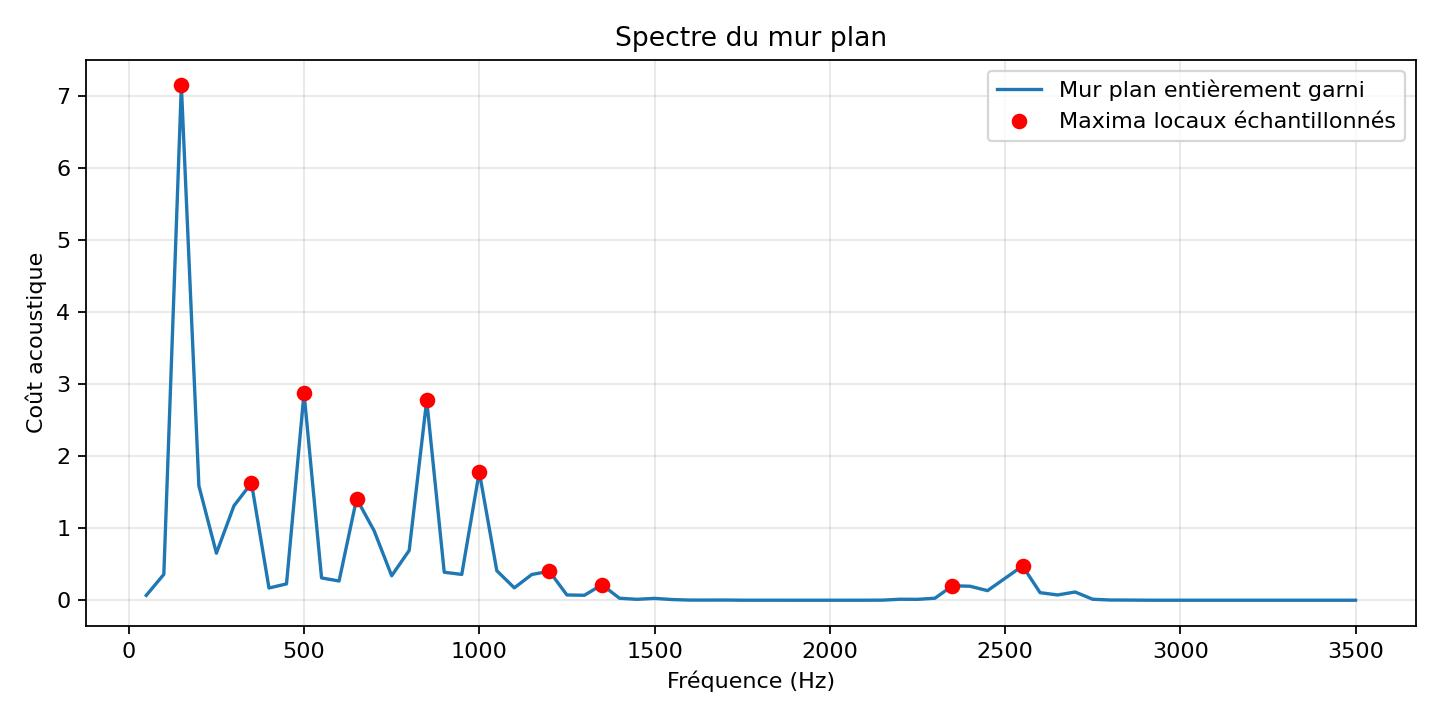
\includegraphics[width=.94\textwidth,height=.36\textheight,keepaspectratio]{resultats_monofrequence/fig_mur_plan_absorbant_maxima.jpg}
\caption{Coût du mur plan entièrement garni en fonction de la fréquence}
\label{fig:murplan}
\end{figure}

Ces pics correspondent aux réponses fortes du domaine avec la paroi poreuse et la source choisies. Leurs positions sont données sur la grille de 50 Hz. La source varie aussi avec la fréquence, donc les courbes regroupent l'effet de l'excitation et celui du dispositif.

\subsection{Effet du niveau géométrique}
La figure~\ref{fig:formes} compare les murs entièrement garnis aux quatre niveaux. L'échelle linéaire met en évidence les pics les plus élevés et l'échelle logarithmique permet de lire les petites valeurs. Les coûts moyens de bande valent \FullCostLevelZero, \FullCostLevelOne, \FullCostLevelTwo{} et \FullCostLevelThree{} pour les niveaux zéro à trois.

\begin{figure}[!htbp]
\centering
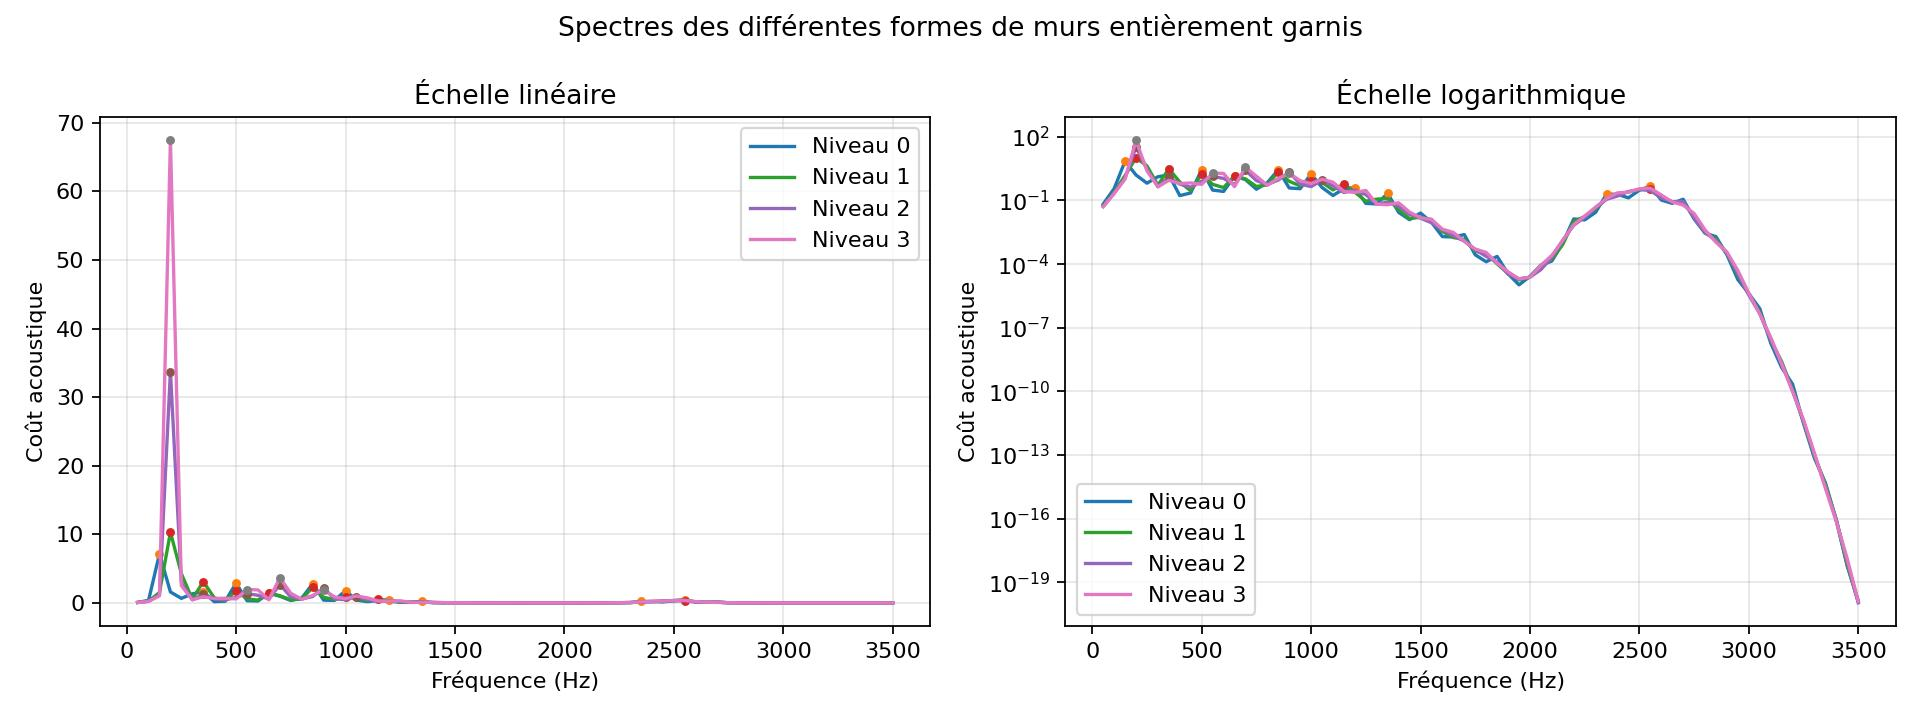
\includegraphics[width=.94\textwidth,height=.30\textheight,keepaspectratio]{resultats_monofrequence/fig_comparaison_formes_fractales.jpg}
\caption{Spectres des murs entièrement garnis aux quatre niveaux}
\label{fig:formes}
\end{figure}

Pour cette source et cette grille, l'allongement du contour n'abaisse donc pas systématiquement le coût. Il modifie les résonances et leur couplage à la source. Les murs entièrement garnis emploient aussi davantage de matériau lorsque le contour s'allonge. Le niveau trois comporte des reliefs de deux pas, ce qui limite l'interprétation de sa courbe.

\subsection{Répartition initiale et recouvrement complet}
La figure~\ref{fig:partiel} compare, pour une même forme, la densité initiale de fraction $0,30$ et la paroi entièrement garnie. \code{project_density} ajuste la quantité de la répartition initiale avant le calcul. Les deux courbes gardent la même source et le même matériau.

\begin{figure}[!htbp]
\centering
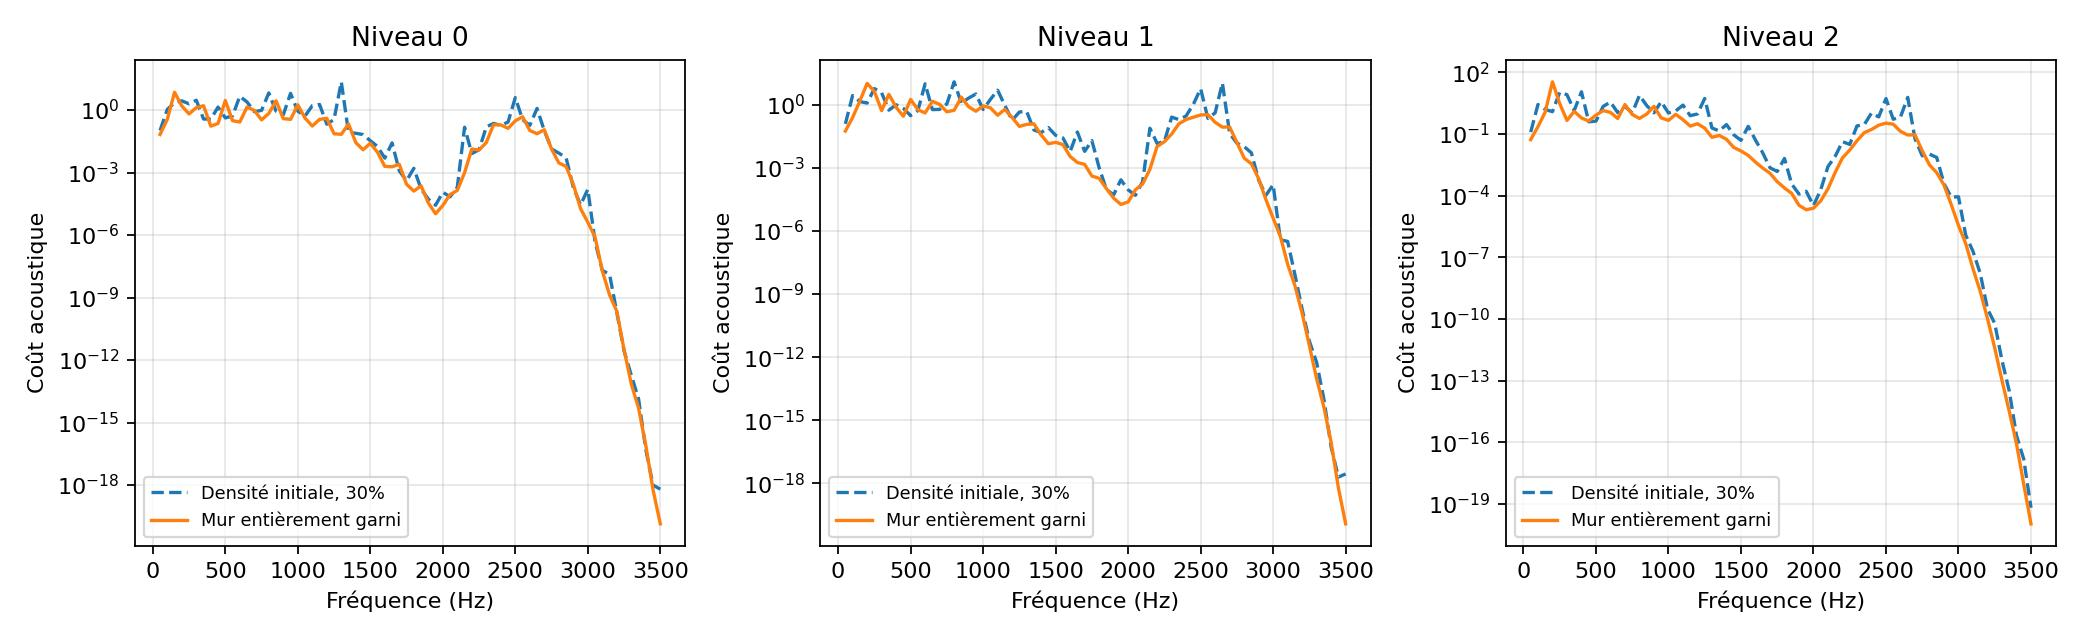
\includegraphics[width=.94\textwidth,height=.28\textheight,keepaspectratio]{resultats_monofrequence/fig_repartition_partielle_et_complete.jpg}
\caption{Spectres du placement initial et du recouvrement complet}
\label{fig:partiel}
\end{figure}

Les courbes montrent les fréquences qui deviennent problématiques avec la quantité réduite. La référence complète utilise 128, 256 ou 512 points garnis selon le niveau, alors que le passage binaire à fraction $0,30$ en emploie 38, 77 ou 154. Elle donne un repère de performance avec une quantité différente.

\subsection{Placement aux fréquences les plus problématiques}
Deux fréquences sont retenues sur le spectre initial de chaque forme. Le tableau~\ref{tab:mono} donne le coût initial, le coût après descente continue, le coût après passage binaire et celui de la paroi entièrement garnie à la même fréquence.
\begin{table}[!htbp]
\centering\small
\begin{tabular}{crrrrrr}
\toprule
Niveau & $f$ (Hz) & $J_{\rm initial}$ & $J_{\rm continu}$ & $J_{\rm binaire}$ & $J_{\rm complet}$ & Étapes\\
\midrule
0 & 800 & 6,661044 & 2,231794 & 2,284860 & 0,690659 & 80\\
0 & 1300 & 22,668078 & 2,197132 & 2,180986 & 0,068720 & 18\\
1 & 800 & 12,189911 & 0,623141 & 0,664143 & 0,541927 & 80\\
1 & 2650 & 10,730143 & 0,111530 & 0,271159 & 0,085859 & 80\\
2 & 250 & 10,437617 & 0,645158 & 0,673449 & 2,953155 & 80\\
2 & 400 & 11,072222 & 0,185310 & 0,186386 & 0,590196 & 80\\
\bottomrule
\end{tabular}

\caption{Coûts aux deux cibles monofréquences de chaque forme}
\label{tab:mono}
\end{table}
La figure~\ref{fig:monohist} montre les historiques de \code{optimize_single_frequency}. Les courbes décroissent pendant les étapes continues acceptées, puis la croix donne le coût binaire recalculé. Le tri final n'a pas le même effet dans tous les cas. Par exemple, au niveau zéro à 1\,300 Hz, le coût passe de $2,197132$ en continu à $2,180986$ en binaire. Pour d'autres cibles il augmente.

\begin{figure}[!htbp]
\centering
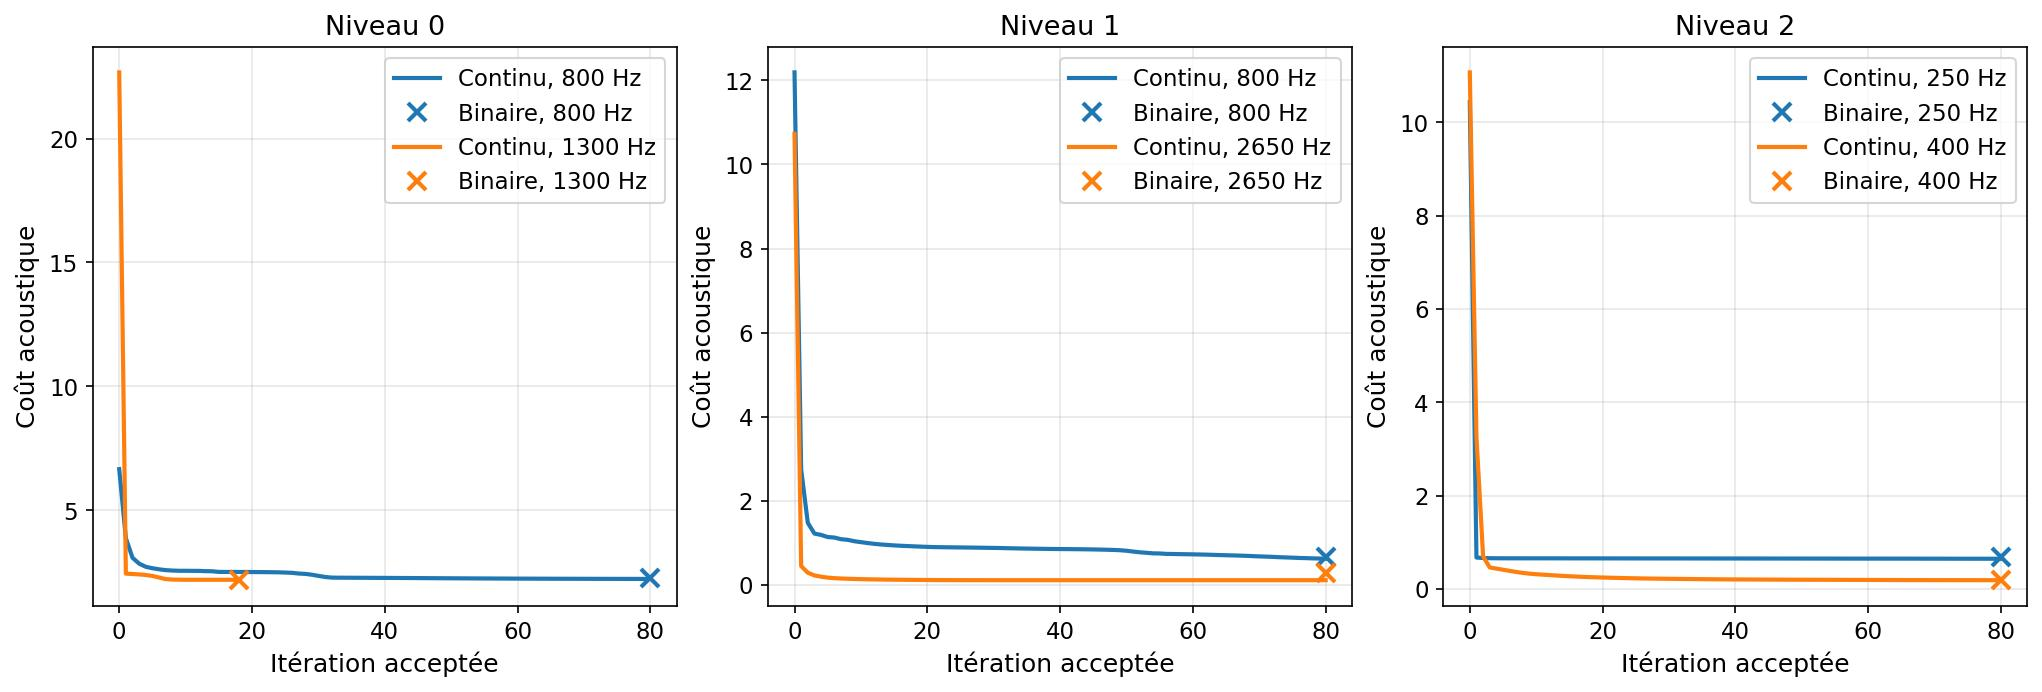
\includegraphics[width=.94\textwidth,height=.28\textheight,keepaspectratio]{resultats_monofrequence/fig_historiques_monofrequence.jpg}
\caption{Coûts continus et binaires des placements monofréquences}
\label{fig:monohist}
\end{figure}

La figure~\ref{fig:monochamps} illustre la première cible du niveau deux, à \MonoExampleFrequency{} Hz. Les cartes initiale et binaire utilisent une même échelle de couleur pour comparer les amplitudes. Le placement final comporte les 154 points garnis prévus après arrondi de la quantité continue $0,30\times512=153,6$. La réduction du coût se lit dans le champ et dans sa somme au carré, et pas seulement dans une renormalisation de la couleur.

\begin{figure}[!htbp]
\centering
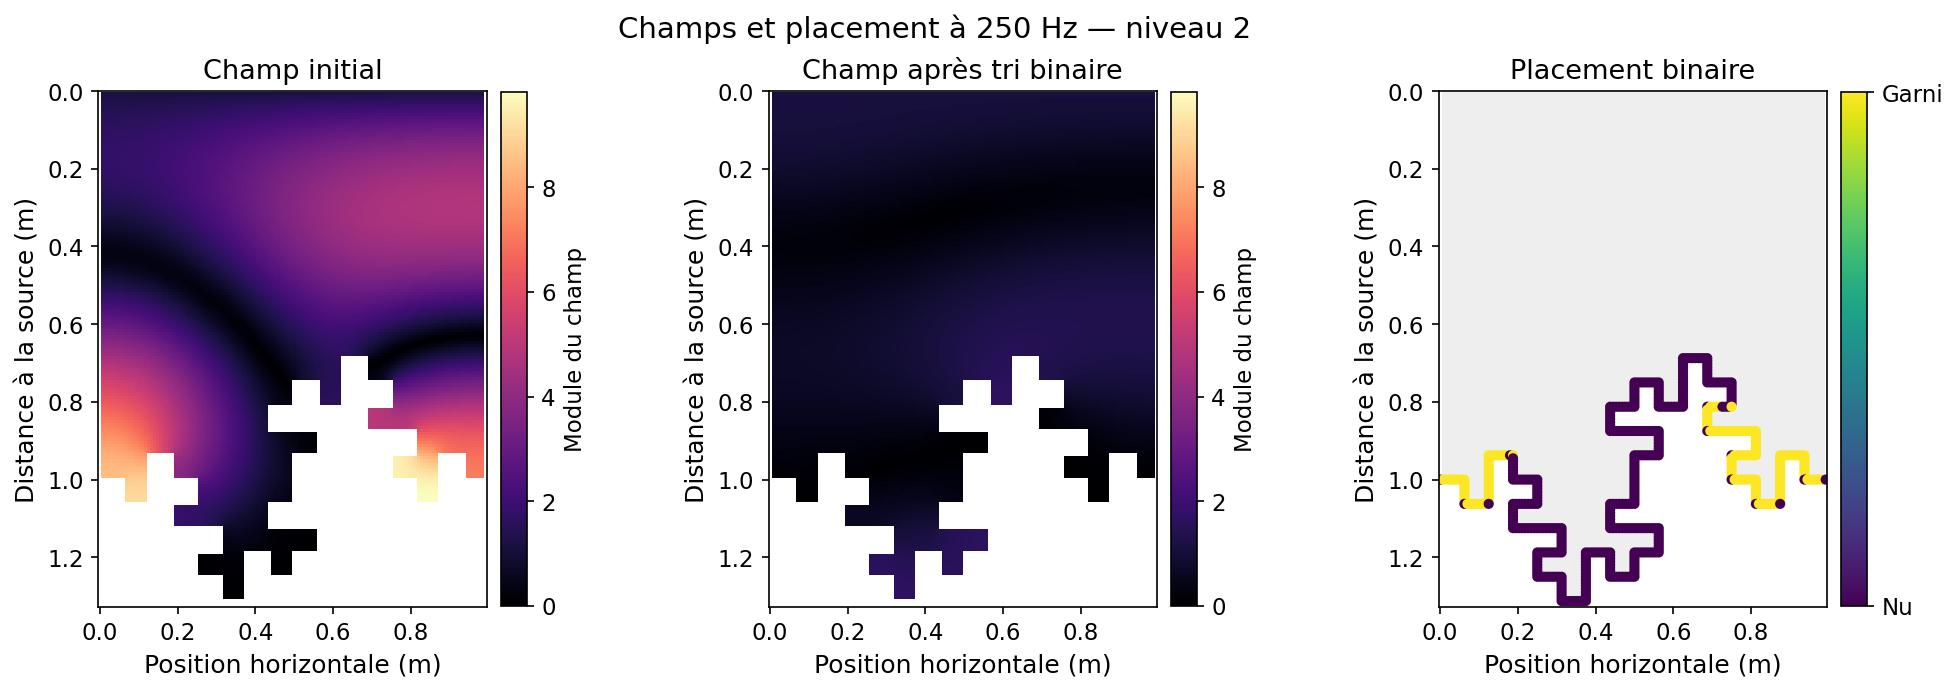
\includegraphics[width=.94\textwidth,height=.30\textheight,keepaspectratio]{resultats_monofrequence/fig_champs_placement_monofrequence.jpg}
\caption{Champs initial et binaire et placement du matériau au niveau deux}
\label{fig:monochamps}
\end{figure}
\section{Placement multifréquence et quantité d’absorbant}
\subsection{Évaluation des placements monofréquences sur la bande}
La fonction \code{evaluate_spectrum} résout le problème sur les 70 fréquences en gardant chaque placement fixe. La figure~\ref{fig:monobande} compare les deux placements monofréquences, le placement initial et la paroi entièrement garnie. Les marqueurs indiquent les fréquences auxquelles chaque placement a été optimisé.

\begin{figure}[!htbp]
\centering
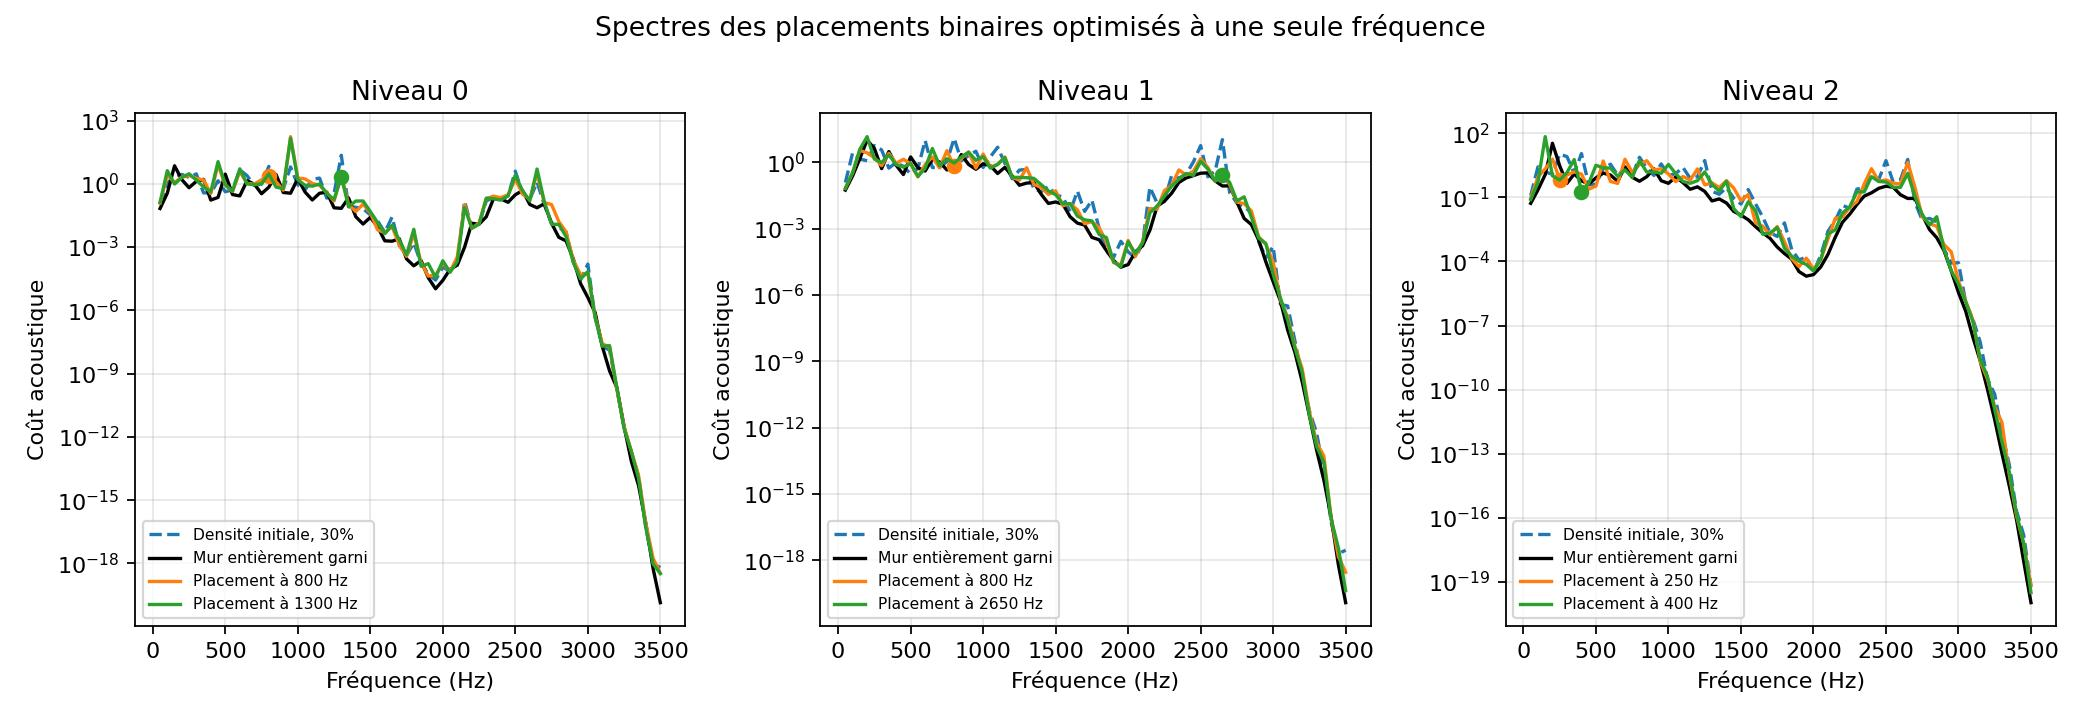
\includegraphics[width=.94\textwidth,height=.29\textheight,keepaspectratio]{resultats_multifrequence/fig_spectres_placements_monofrequence.jpg}
\caption{Spectres des placements optimisés à une seule fréquence}
\label{fig:monobande}
\end{figure}

Une baisse du coût à la cible peut s'accompagner d'une hausse ailleurs. Le tableau de données conserve donc, en plus des coûts aux cibles, la moyenne sur toute la bande. Cette vérification motive la recherche d'une même répartition pour plusieurs fréquences.

\subsection{Optimisation simultanée de trois fréquences}
\code{study_multifrequency_placement_and_coverage} organise cette étude.

On sélectionne trois cibles par forme, puis \code{optimize_multi_frequency} minimise le critère \eqref{eq:multi}. Le tableau~\ref{tab:multi} indique les cibles et les coûts moyens continu et binaire sur ces cibles.
\begin{table}[!htbp]
\centering\small
\begin{tabular}{clrrrr}
\toprule
Niveau & Cibles (Hz) & $J_{\rm initial}$ & $J_{\rm continu}$ & $J_{\rm binaire}$ & $J_{\rm complet}$\\
\midrule
0 & 800, 950, 1300 & 11,883442 & 1,158950 & 4,963280 & 0,372361\\
1 & 600, 800, 2650 & 10,916475 & 0,398085 & 0,556211 & 0,344168\\
2 & 250, 400, 800 & 9,653963 & 0,501330 & 0,521403 & 1,368547\\
\bottomrule
\end{tabular}

\caption{Fréquences cibles et coûts de l’optimisation multifréquence}
\label{tab:multi}
\end{table}
La figure~\ref{fig:multihist} détaille le niveau deux. Chaque courbe fine donne le coût d'une fréquence, tandis que la courbe pointillée représente leur moyenne. La descente impose la baisse de cette moyenne, donc une composante peut augmenter à une étape si les autres diminuent davantage.

\begin{figure}[!htbp]
\centering
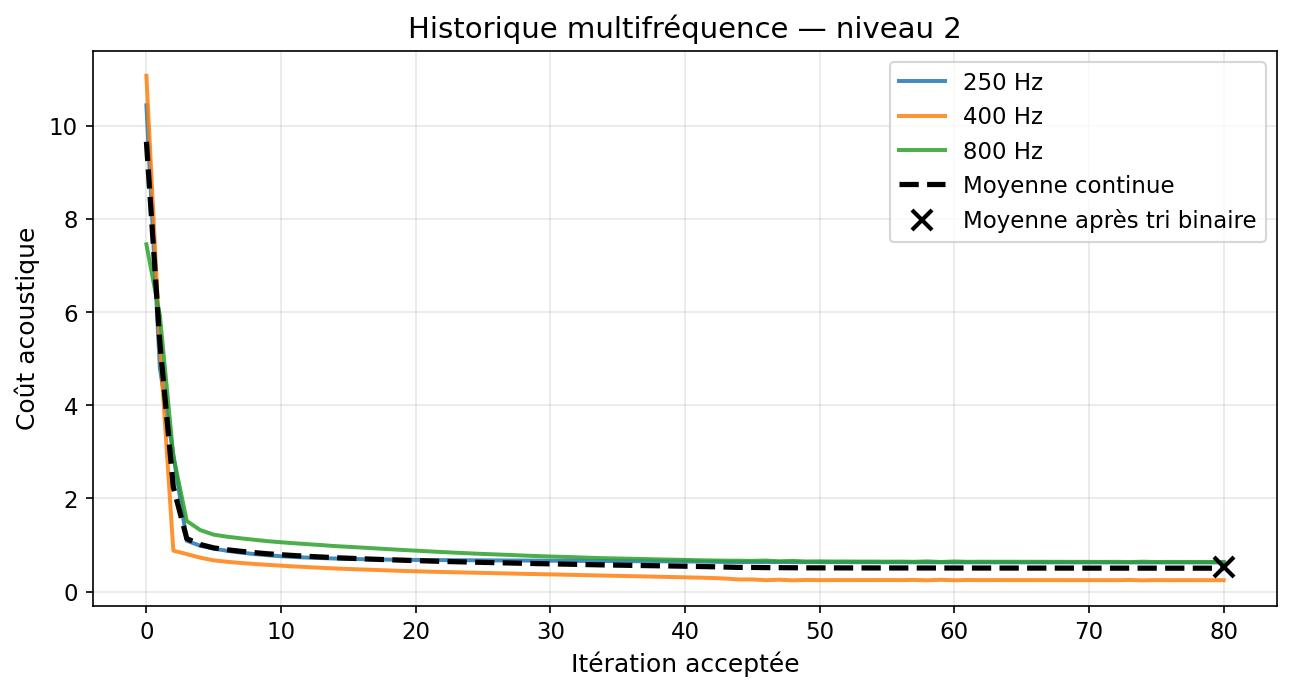
\includegraphics[width=.94\textwidth,height=.36\textheight,keepaspectratio]{resultats_multifrequence/fig_historique_multifrequence.jpg}
\caption{Coûts des trois cibles et de leur moyenne au niveau deux}
\label{fig:multihist}
\end{figure}

Le passage binaire doit de nouveau être mesuré. Au niveau zéro, le coût moyen sur les cibles passe de $1,158950$ pour la densité continue à $4,963280$ pour la densité binaire. Le tri des densités ne conserve donc pas nécessairement le compromis obtenu par l'optimisation continue.

La figure~\ref{fig:multibande} présente les spectres du niveau deux avec les différents placements. La moyenne de bande du placement multifréquence binaire vaut \MultiBandLevelTwo, contre \InitialBandLevelTwo{} pour le placement initial et \FullCostLevelTwo{} pour la paroi entièrement garnie. Les résultats aux trois niveaux figurent dans les données numériques associées.

\begin{figure}[!htbp]
\centering
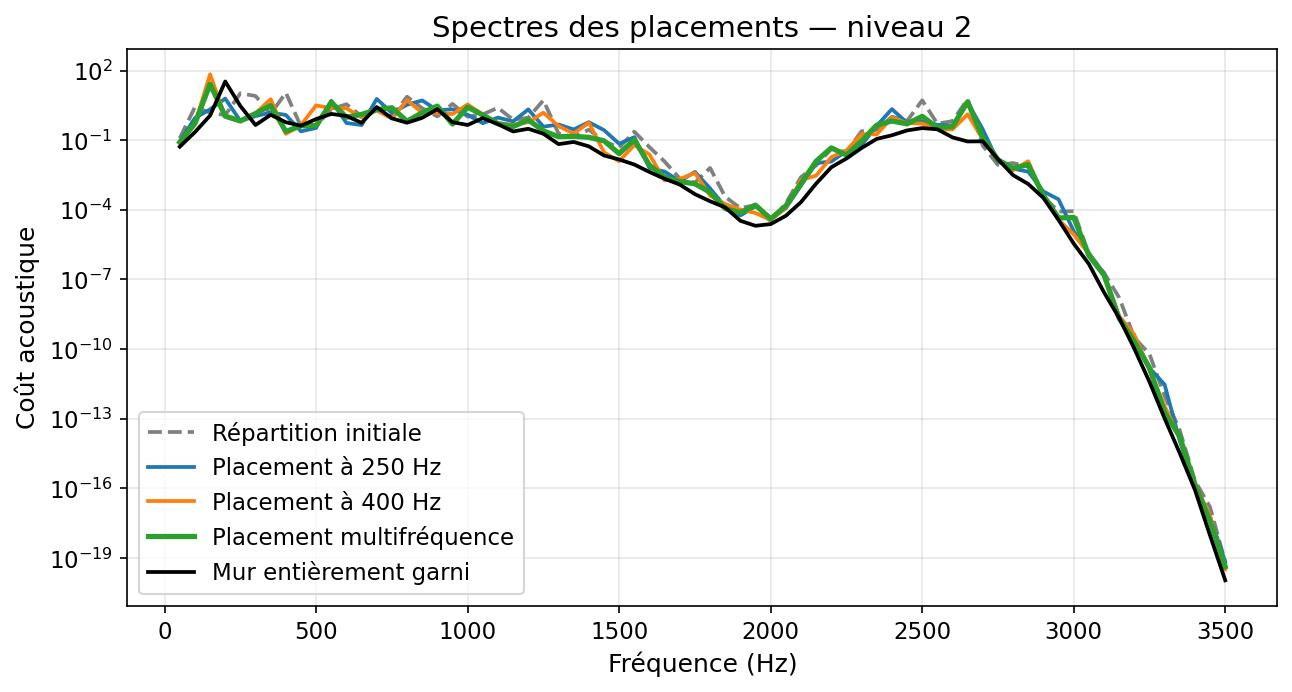
\includegraphics[width=.94\textwidth,height=.36\textheight,keepaspectratio]{resultats_multifrequence/fig_spectre_multifrequence.jpg}
\caption{Spectres initial, monofréquences, multifréquence et entièrement garni au niveau deux}
\label{fig:multibande}
\end{figure}

\subsection{Influence de la quantité de matériau}
Pour chaque forme, on répète les optimisations avec les fractions $0,10$, $0,30$, $0,50$, $0,70$ et un. La figure~\ref{fig:quantite} présente les coûts binaires obtenus à une fréquence, puis sur les trois fréquences. Les cibles d'une même forme restent fixes quand la quantité change. La fraction un donne directement le mur entièrement garni.

\begin{figure}[!htbp]
\centering
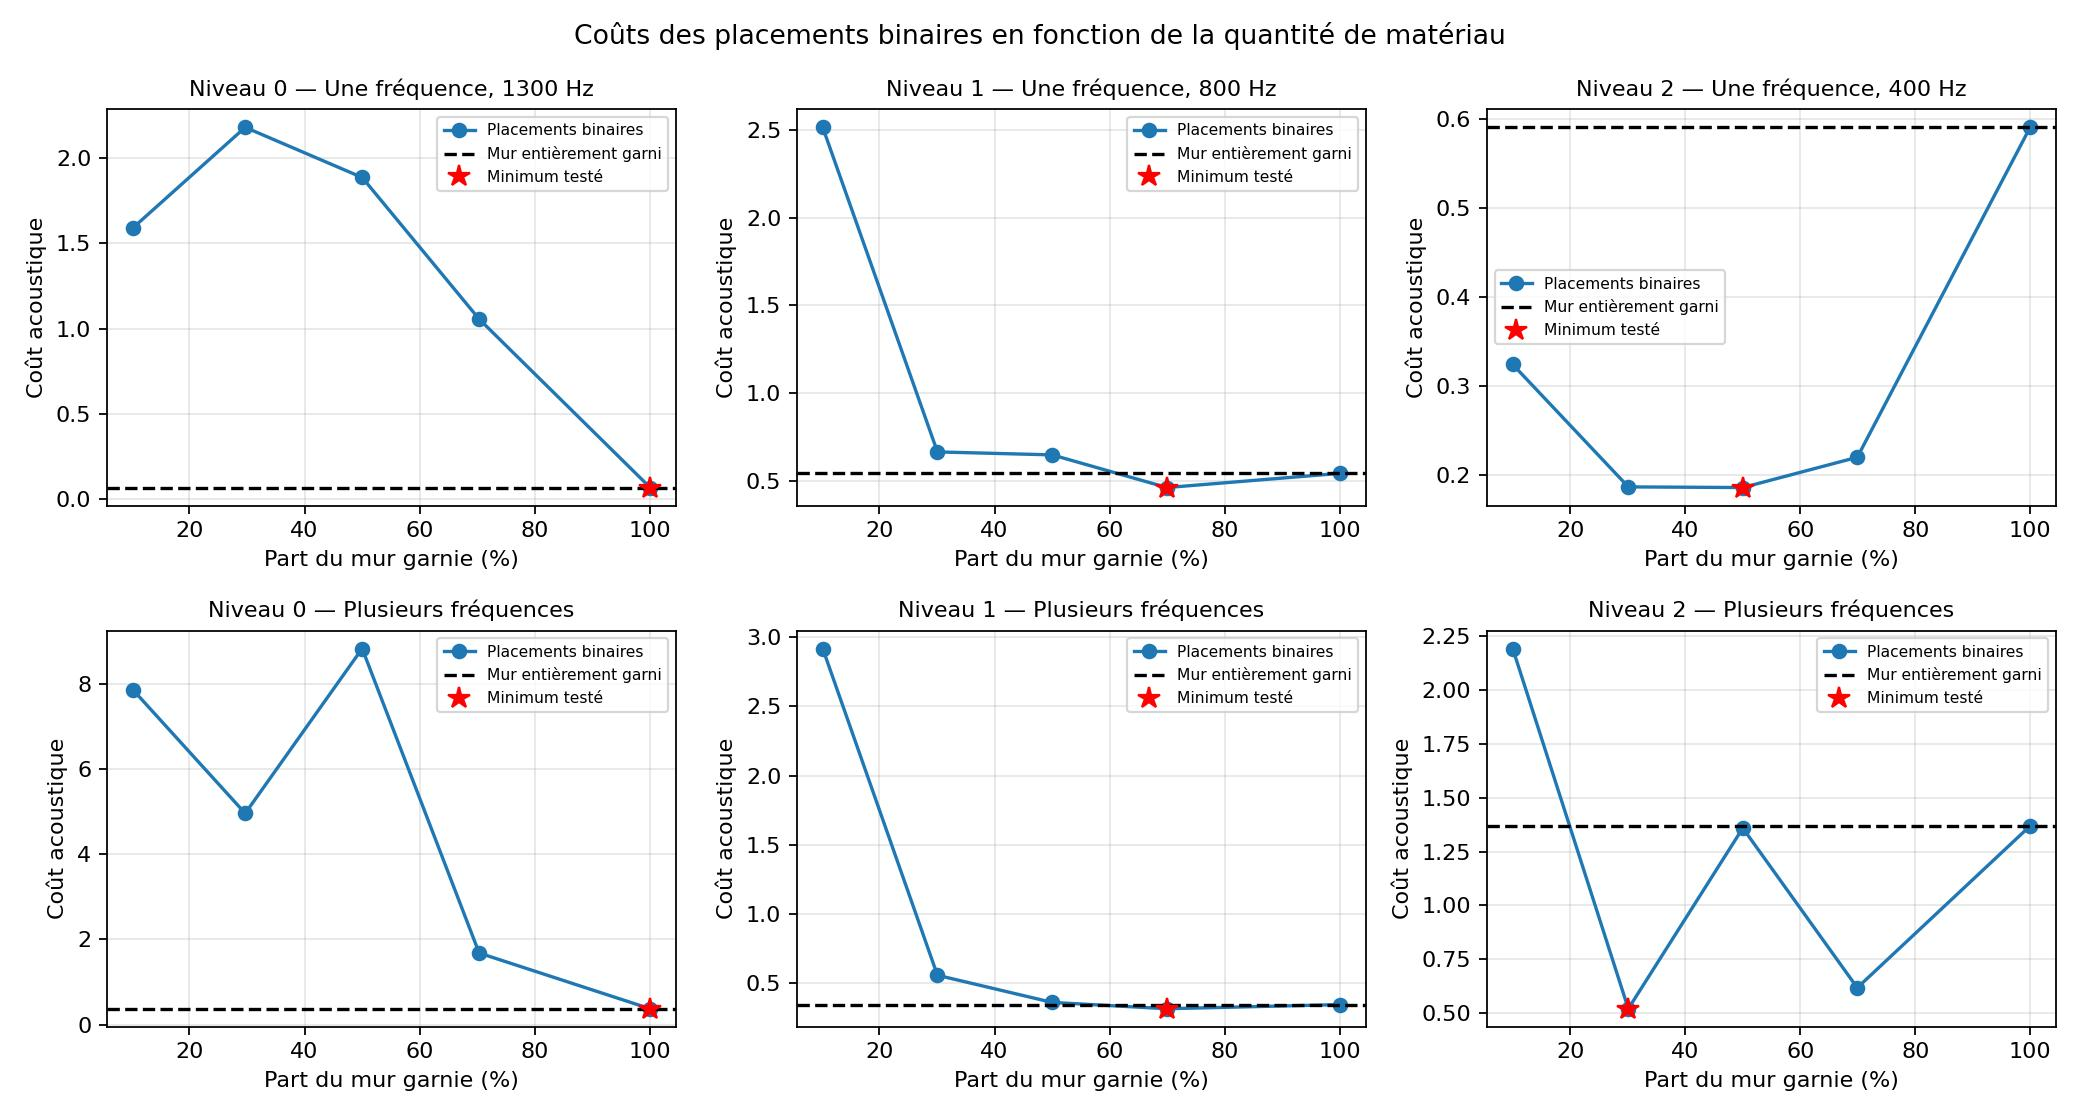
\includegraphics[width=.94\textwidth,height=.37\textheight,keepaspectratio]{resultats_multifrequence/fig_cout_quantite_absorbant.jpg}
\caption{Coût binaire en fonction de la fraction de points garnis}
\label{fig:quantite}
\end{figure}

Le mur plan atteint le coût le plus faible à $100\,\%$ pour les deux critères testés. Au niveau un, le meilleur résultat est obtenu à $70\,\%$, avec des coûts $0,460803$ à 800 Hz et $0,314059$ sur les trois cibles, contre $0,541927$ et $0,344168$ pour le recouvrement complet. Au niveau deux, le minimum monofréquence est observé à $50\,\%$, avec $J_h=0,185653$ à 400 Hz, et le minimum multifréquence à $30\,\%$, avec une moyenne $0,521403$, contre $1,368547$ pour le mur entièrement garni sur ces mêmes trois cibles.

Le minimum indiqué correspond aux quantités testées et aux placements trouvés par la descente. Les fréquences utilisées dans les deux lignes de la figure sont différentes selon le critère, donc les ordonnées ne se comparent pas directement d'une ligne à l'autre. À quantité fixée, des points de départ ou des répartitions binaires différents peuvent aussi donner d'autres valeurs.
\section{Comparaison des dispositifs et choix retenu}
\subsection{Densité continue, placement binaire et mélange de matériaux}
La fonction \code{compare_absorber_configurations} reprend le niveau deux avec le matériau de référence. Les trois fréquences sont choisies dans le spectre initial de ce niveau et servent aux comparaisons finales. Une seconde matière est placée sur la partie basse des points déjà sélectionnés, pour tester un mélange prescrit de laine de roche et de mélamine. Cette répartition à deux matériaux est évaluée séparément.

La figure~\ref{fig:mixte} montre les spectres initial, continu, binaire, mixte et entièrement garni. Les moyennes de bande sont respectivement \ConfigInitialBand, \ConfigContinuousBand, \ConfigBinaryBand, \ConfigMixedBand{} et \ConfigFullBand. Le résultat du mélange se juge sur la courbe calculée, sans supposer que deux matériaux soient toujours plus efficaces qu'un seul.

\begin{figure}[!htbp]
\centering
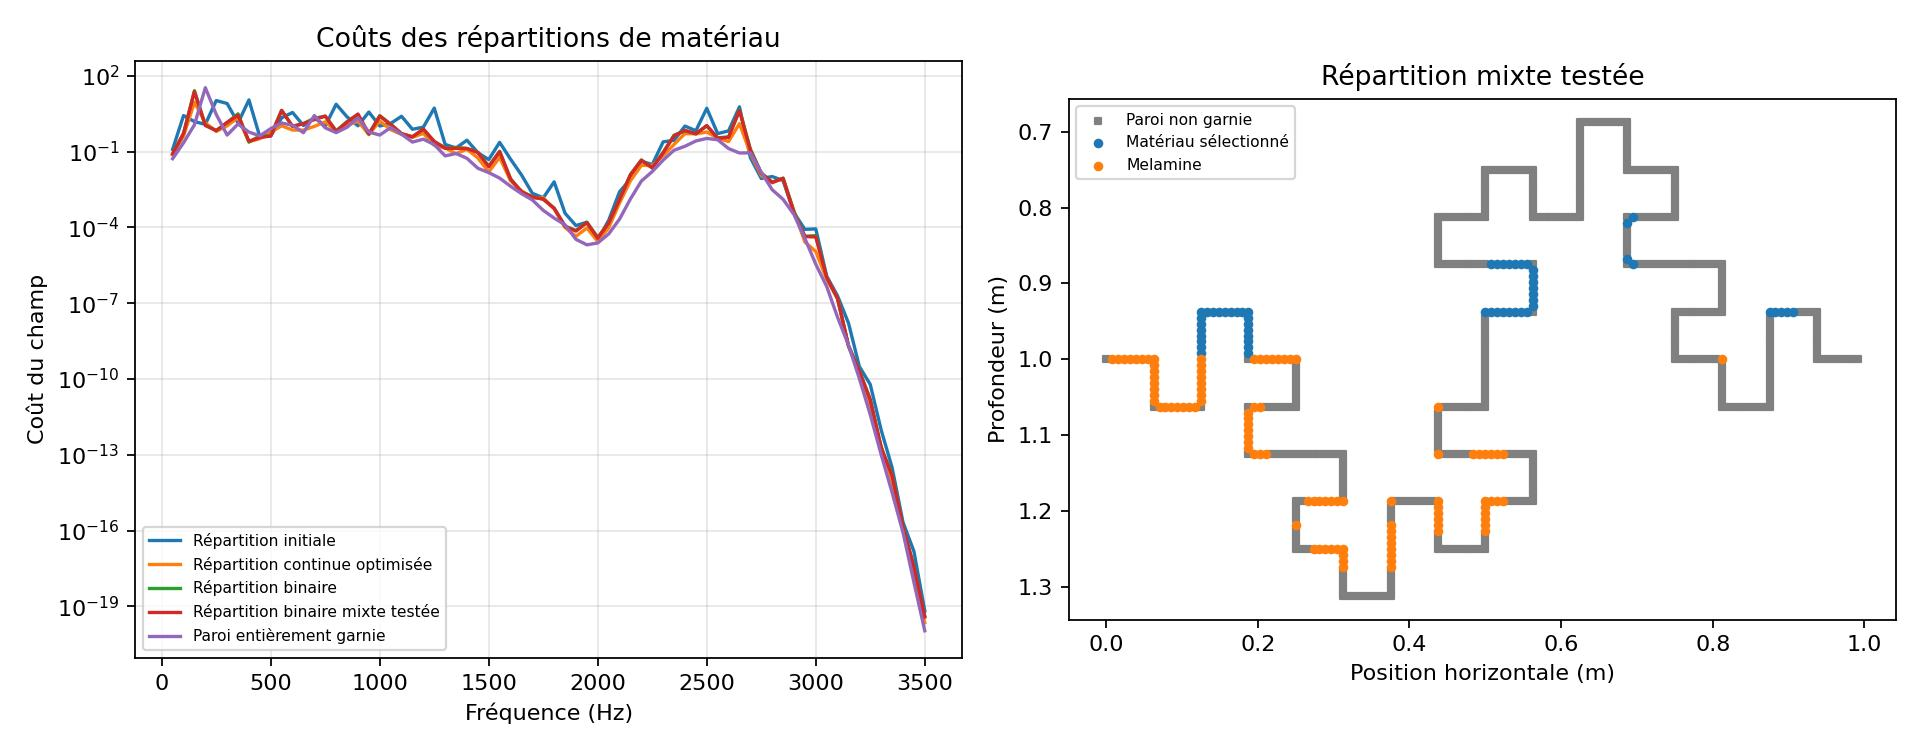
\includegraphics[width=.94\textwidth,height=.31\textheight,keepaspectratio]{resultats_comparaison_dispositifs/fig_repartitions_binaire_et_mixte.jpg}
\caption{Spectres des répartitions et emplacement des deux matériaux}
\label{fig:mixte}
\end{figure}

\subsection{Effet du profil de l’excitation}
À \ProfileFrequency{} Hz, on garde la même paroi et les mêmes coefficients pour comparer trois profils d'entrée. Le profil uniforme impose la même valeur sur tous les points. Le profil localisé excite un seul point au centre du bord. Le profil oblique impose une phase variant avec la position, avec un angle de $35^\circ$.

Chaque profil est normalisé pour conserver la même somme des modules au carré sur le bord de Dirichlet. La figure~\ref{fig:profils} compare le champ initial et le champ obtenu avec le placement binaire. Les deux cartes d'un même profil ont une échelle de couleur commune. Le test examine l'effet de la répartition spatiale de la source avec un coefficient de matériau conservé.

\begin{figure}[!htbp]
\centering
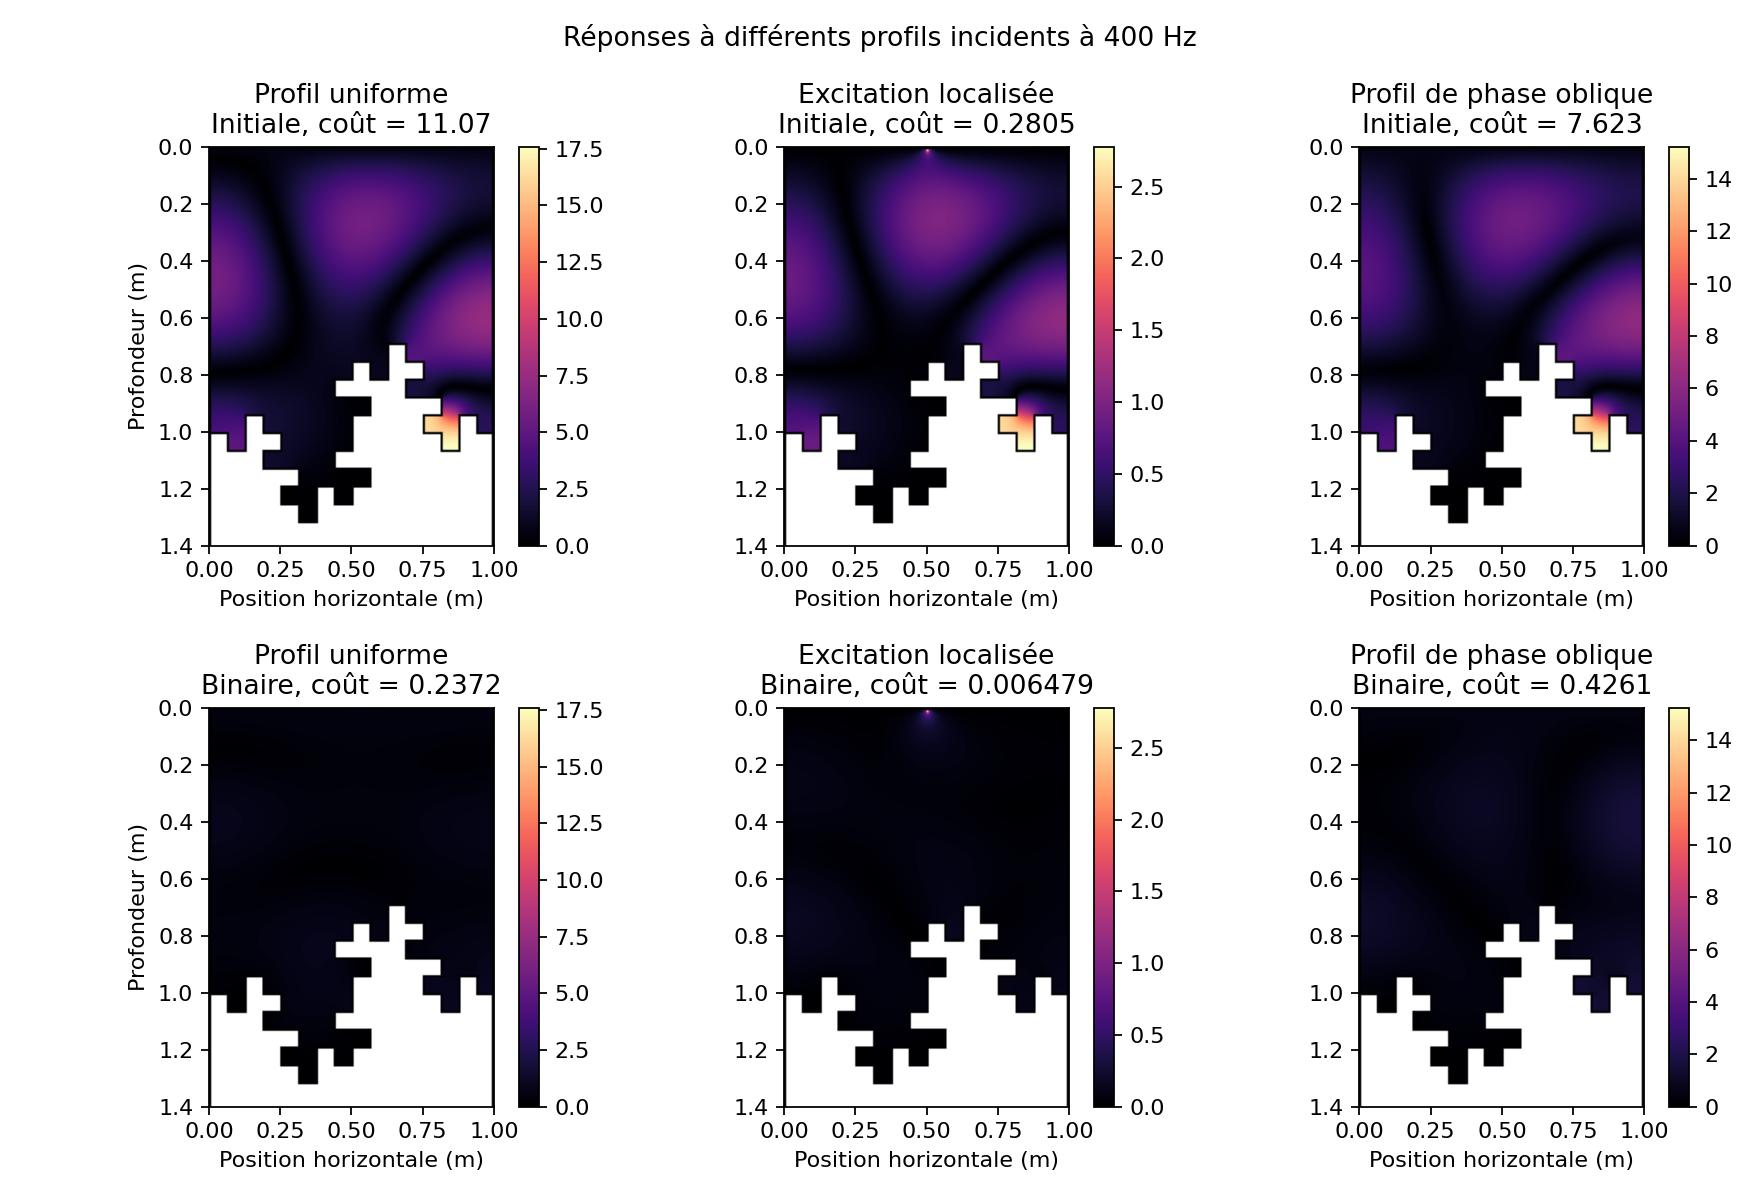
\includegraphics[width=.94\textwidth,height=.37\textheight,keepaspectratio]{resultats_comparaison_dispositifs/fig_comparaison_profils_sources.jpg}
\caption{Champs initial et binaire pour trois profils d’entrée}
\label{fig:profils}
\end{figure}

Les coûts initial et binaire valent respectivement $11,072222$ et $0,237224$ pour le profil uniforme, puis $0,280499$ et $0,006479$ pour le profil localisé, puis $7,622802$ et $0,426138$ pour le profil oblique. Le placement binaire réduit ici le coût pour les trois profils. Les valeurs et les cartes confirment néanmoins que la réponse dépend du profil d’entrée.

La normalisation choisie permet une comparaison des données de bord du modèle. Les trois profils ne représentent pas des flux acoustiques réels étalonnés. Les différences de champ montrent néanmoins pourquoi un placement construit pour une excitation uniforme doit être réévalué lorsque cette excitation change.

\subsection{Comparaison à budget nodal commun}
Une fraction de $0,30$ représente 38, 77 ou 154 points garnis après arrondi selon la forme. Pour choisir entre les formes, on complète ce premier calcul par un budget identique de 38 points. Les fractions des niveaux zéro, un et deux sont alors $0,296875$, $0,1484375$ et $0,07421875$. Le budget $Q_h$ de \eqref{eq:budget}, la source, les trois cibles et les 70 fréquences d'évaluation sont communs.

Les trois placements du mur plan calculés précédemment à fraction $0,30$ ont déjà 38 points garnis après le tri. On conserve aussi ces solutions admissibles. Leur contrainte continue vaut $38,4$ points au lieu de 38, ce qui peut modifier la trajectoire de descente et le résultat du tri. La fonction \code{combine_comparable_configurations} retient, pour chaque couple forme--matériau, le coût moyen binaire le plus faible parmi les répartitions disponibles à 38 points. Au total, 12 répartitions admissibles alimentent les neuf couples du classement. Cette comparaison met en évidence la sensibilité du résultat à la recherche continue et à son passage binaire.

La figure~\ref{fig:budget} compare les neuf couples forme--matériau. On utilise les placements binaires recalculés et la moyenne sur toute la bande, après une optimisation visant les trois fréquences communes. Chaque référence entièrement garnie emploie sa quantité propre. Le tableau~\ref{tab:candidats} conserve aussi le coût maximal échantillonné, qui peut conduire à un autre choix que la moyenne.

\begin{figure}[!htbp]
\centering
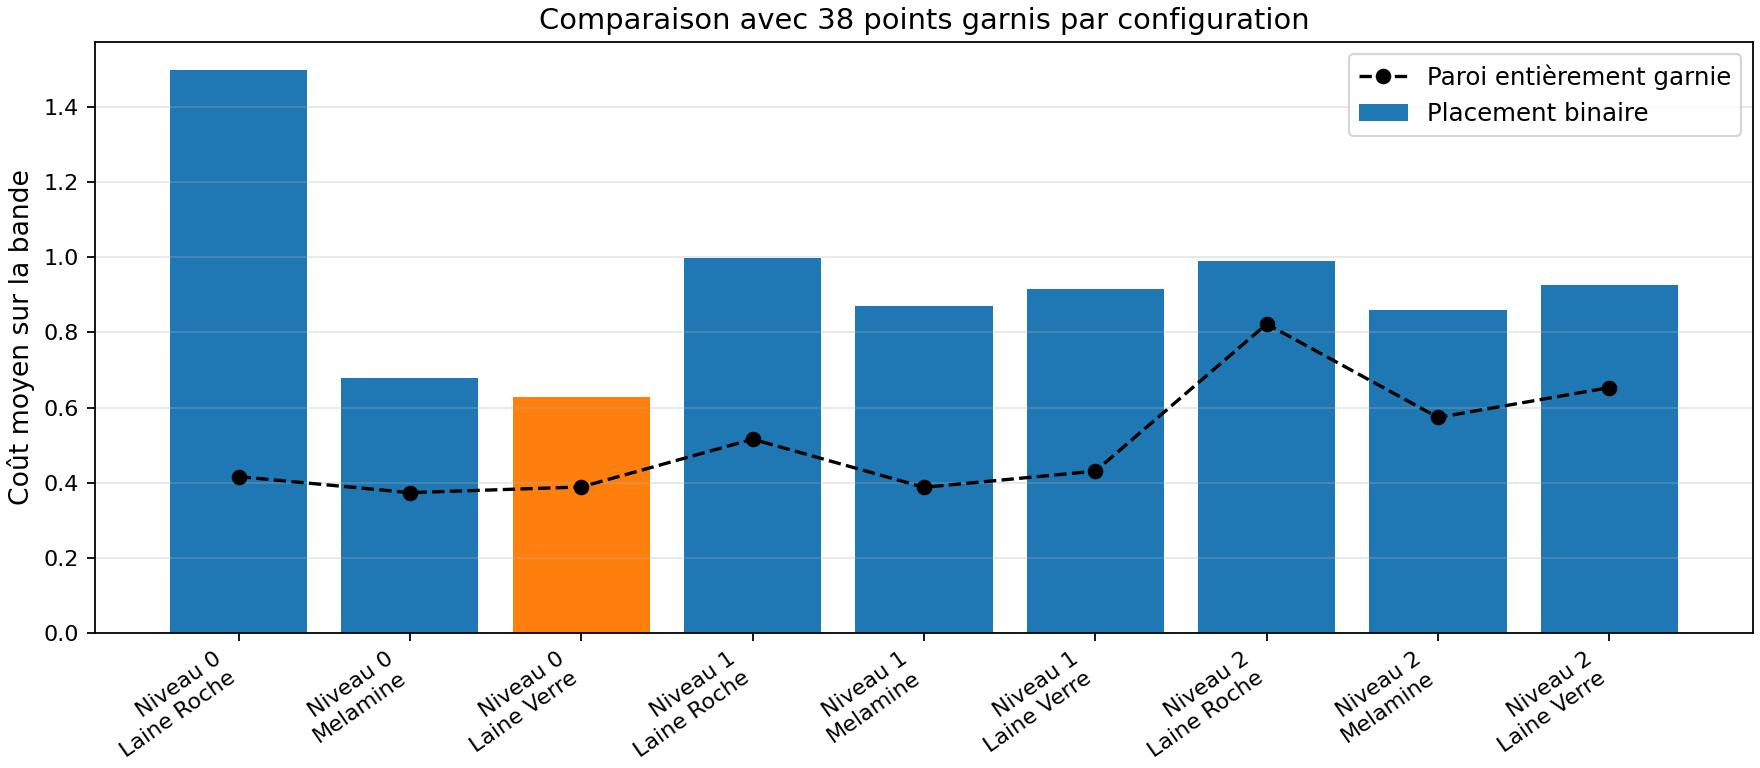
\includegraphics[width=.94\textwidth,height=.31\textheight,keepaspectratio]{resultats_comparaison_dispositifs/fig_comparaison_budget_identique.jpg}
\caption{Coûts moyens des neuf configurations à budget identique}
\label{fig:budget}
\end{figure}

\begin{table}[!htbp]
\centering\small
\begin{tabular}{clrrr}
\toprule
Niveau & Matériau & $\overline J_{\rm binaire}$ & $J_{\rm max}$ & $\overline J_{\rm complet}$\\
\midrule
0 & Laine de roche & 1,498210 & 22,851874 & 0,416078\\
0 & Mélamine & 0,679267 & 7,270847 & 0,373342\\
0 & Laine de verre & 0,627376 & 9,126397 & 0,388505\\
1 & Laine de roche & 0,999343 & 9,301208 & 0,515656\\
1 & Mélamine & 0,870016 & 11,685023 & 0,387483\\
1 & Laine de verre & 0,914874 & 10,775739 & 0,430512\\
2 & Laine de roche & 0,990891 & 8,797360 & 0,822255\\
2 & Mélamine & 0,859505 & 8,648555 & 0,573583\\
2 & Laine de verre & 0,926069 & 9,881990 & 0,653067\\
\bottomrule
\end{tabular}

\caption{Coûts des configurations binaires avec 38 points garnis}
\label{tab:candidats}
\end{table}
Pour minimiser la moyenne sur la bande, on retient le mur plan en laine de verre, avec 38 points garnis sur 128. Son coût moyen vaut $0,627376$ et son maximum échantillonné $9,126397$. Si l'objectif prioritaire est de réduire le maximum, le mur plan en mélamine donne $7,270847$, avec une moyenne $0,679267$. Le critère de choix doit donc être annoncé.

La figure~\ref{fig:retenu} compare le placement retenu à un placement initial binaire de même quantité et à la paroi entièrement garnie. \code{evaluate_selected_configuration} reconstruit ce contrôle à partir des données du candidat. La moyenne initiale vaut $1,279166$ et le maximum initial $37,344859$, d'où des réductions respectives de $50,95\,\%$ et $75,56\,\%$. Ces gains comparent la même source, le même matériau, la même forme et le même nombre de points garnis.
\begin{figure}[!htbp]
\centering
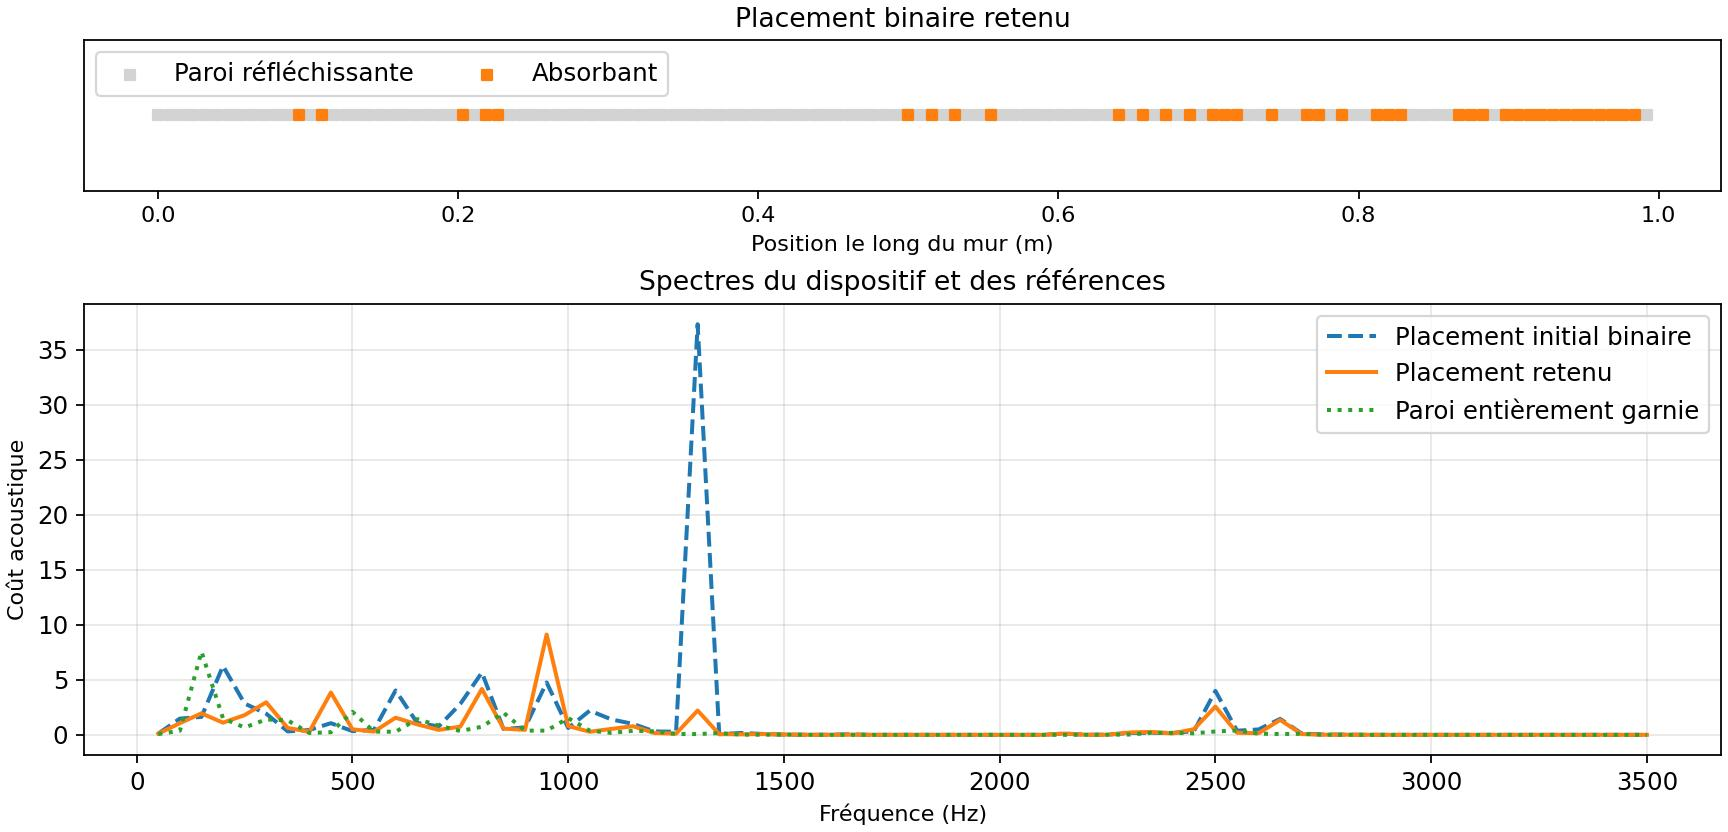
\includegraphics[width=.96\textwidth,height=.33\textheight,keepaspectratio]{resultats_comparaison_dispositifs/fig_dispositif_retenu.jpg}
\caption{Placement retenu et spectres des trois références de laine de verre}
\label{fig:retenu}
\end{figure}

La référence entièrement garnie a une moyenne $0,388505$. Le candidat utilise $70,31\,\%$ de points garnis en moins et son coût moyen est $61,48\,\%$ plus élevé que celui de cette référence. Il représente donc un compromis à budget réduit, avec un gain établi par rapport au placement initial de même quantité.

Ce choix concerne les formes et matériaux testés, la source retenue et ce budget discret. Il fournit un candidat de développement à partir des résultats du modèle. La fabrication demande de traduire les points garnis en portions physiques suffisamment résolues, puis d'évaluer la géométrie et les matériaux avec des données adaptées au site ferroviaire.
\section*{Conclusion}
\addcontentsline{toc}{section}{Conclusion}
Le projet a relié le choix de la source, le calcul du coefficient de paroi et l'optimisation du placement d'absorbant. Les références ouverte et réfléchissante ont permis de vérifier le comportement du modèle, puis le contrôle par différences centrées a confirmé le gradient utilisé. Les spectres montrent que l'effet de la forme dépend de la fréquence et que l'augmentation du contour ne suffit pas à prévoir le coût obtenu.

L'optimisation monofréquence améliore la réponse à sa cible, d'où l'intérêt d'examiner ensuite toute la bande. L'optimisation multifréquence recherche un compromis commun à quelques fréquences, mais le passage binaire peut modifier ce compromis. Les coûts sont donc recalculés pour la répartition effectivement retenue. Le balayage des quantités complète cette analyse en distinguant le meilleur résultat parmi les fractions testées d'un optimum sur toutes les quantités possibles.

À budget de 38 points garnis, le candidat de plus faible moyenne de bande est le niveau \RecommendedLevel{} avec \RecommendedMaterial. Sa moyenne vaut \RecommendedBandCost{} dans les unités relatives du modèle. Ce résultat guide le choix de ResoniCS pour les conditions calculées. Les petits reliefs, les portions garnies et le pas fréquentiel restent à examiner plus finement pour passer du candidat numérique à un dimensionnement physique.

\clearpage
\begin{thebibliography}{99}
\bibitem{lee2022}
H.~P. Lee, S.~Kumar, S.~Garg et K.~M. Lim.
\emph{Comparison of Cabin Noise of Airport Express Rail Systems}.
\emph{Acoustics}, 4(1), 1--13, 2022.
\href{https://doi.org/10.3390/acoustics4010001}{doi:10.3390/acoustics4010001}.

\bibitem{metro2026}
L.~Song, Z.~Wang, P.~Zhang, Q.~Liu et B.~Bai.
\emph{Noise from Different Metro Train Types on Elevated Tracks: A Case Study Based on Field Measurements}.
\emph{Buildings}, 16(6), 1191, 2026.
\href{https://doi.org/10.3390/buildings16061191}{doi:10.3390/buildings16061191}.

\bibitem{kim2019}
J.~C. Kim, Y.~S. Yun et H.-M. Noh.
\emph{Analysis of Wheel Squeal and Flanging on Curved Railway Tracks}.
\emph{International Journal of Precision Engineering and Manufacturing}, 20, 2077--2087, 2019.
\href{https://doi.org/10.1007/s12541-019-00225-7}{doi:10.1007/s12541-019-00225-7}.

\bibitem{cours}
A.~Rozanova-Pierrat.
\emph{Contrôle des Ondes}.
Polycopié de cours, CentraleSupélec, 4 septembre 2026.

\bibitem{filoche}
M.~Filoche.
\emph{Waves next to irregular boundaries --- Wave localization, absorption, and noise abatement wall}.
Présentation pédagogique fournie pour le projet.

\bibitem{sota}
Équipe ResoniCS.
\emph{État de l'art : RER B}.
Synthèse de travail interne, 2026.
\bibitem{sncfbruit}
Groupe SNCF.
\emph{Nos engagements pour la réduction du bruit ferroviaire}.
Entretien avec Jean-Philippe Regairaz, SNCF Réseau, mis à jour le 20 février 2026.
\url{https://www.groupe-sncf.com/fr/engagements/developpement-durable/ressources-biodiversite/interview-reduire-bruit-ferroviaire}

\bibitem{quierail}
DELTABLOC.
\emph{PHONOBLOC --- Série Special Rail : écrans acoustiques en bordure de voie ferrée}.
Documentation du fabricant, consultée le 2 novembre 2026.
\url{https://deltabloc.com/fr/produits/phonobloc/serie-special-rail}

\bibitem{metawindow}
Phononic Vibes.
\emph{Rail --- MetaWindow}.
Présentation du fabricant, consultée le 2 novembre 2026.
\url{https://phononic-vibes.com/markets/rail/}

\bibitem{felix2009}
S.~Félix, B.~Sapoval, M.~Filoche et M.~Asch.
\emph{Enhanced wave absorption through irregular interfaces}.
EPL, 85, article 14003, 2009.
\href{https://doi.org/10.1209/0295-5075/85/14003}{doi:10.1209/0295-5075/85/14003}.
\href{https://www.institut-langevin.espci.fr/biblio/2024/8/21/2179/files/EPL_2009.pdf}{Texte intégral en accès libre}.

\bibitem{magoules2021}
F.~Magoulès, T.~P. Kieu Nguyen, P.~Omnes et A.~Rozanova-Pierrat.
\emph{Optimal Absorption of Acoustic Waves by a Boundary}.
SIAM Journal on Control and Optimization, 59(1), 561--583, 2021.
\href{https://doi.org/10.1137/20M1327239}{doi:10.1137/20M1327239}.
\href{https://arxiv.org/abs/2003.13250}{Version auteur en accès libre}.

\bibitem{magoules2025}
F.~Magoulès, M.~Menoux et A.~Rozanova-Pierrat.
\emph{Frequency Range of a Non-Lipschitz Parametric Optimization of a Noise Absorption}.
SIAM Journal on Control and Optimization, 63(2), 1267--1285, 2025.
\href{https://doi.org/10.1137/24M1691296}{doi:10.1137/24M1691296}.
\href{https://arxiv.org/abs/2409.06292}{Version auteur en accès libre}.

\end{thebibliography}
\end{document}
